\documentclass[preprint,12pt,authoryear]{elsarticle}

\usepackage{amsmath,amssymb,amsfonts}
\usepackage{amsthm}
\usepackage{mathrsfs}
\usepackage{graphicx}
\usepackage{booktabs}
\usepackage[section]{placeins}
% Generated by manuscript/make_numbers.py -- do not edit by hand.
% Every value below is read from real_data/results_*.json.

\newcommand{\nGptComp}{72}
\newcommand{\nGptNeg}{24}
\newcommand{\nGptBenign}{70}
\newcommand{\GptSthreeAuroc}{0.951}
\newcommand{\GptSthreeAurocSd}{0.026}
\newcommand{\GptSthreeTpr}{0.661}
\newcommand{\GptSthreeTprSd}{0.433}
\newcommand{\GptSthreeFpr}{1.2}
\newcommand{\GptSthreeTprLow}{0.472}
\newcommand{\GptSthreeFprLow}{0.0}
\newcommand{\GptSfourAuroc}{0.900}
\newcommand{\GptSfourAurocSd}{0.039}
\newcommand{\GptSfourTpr}{0.267}
\newcommand{\GptSfourTprSd}{0.407}
\newcommand{\GptSfourFpr}{0.4}
\newcommand{\GptSfourTprLow}{0.178}
\newcommand{\GptSfourFprLow}{0.0}
\newcommand{\GptSfiveAuroc}{0.868}
\newcommand{\GptSfiveAurocSd}{0.019}
\newcommand{\GptSfiveTpr}{0.164}
\newcommand{\GptSfiveTprSd}{0.328}
\newcommand{\GptSfiveFpr}{0.4}
\newcommand{\GptSfiveTprLow}{0.082}
\newcommand{\GptSfiveFprLow}{0.0}
\newcommand{\GptSoneAuroc}{0.481}
\newcommand{\GptSoneAurocSd}{0.062}
\newcommand{\GptSoneTpr}{0.000}
\newcommand{\GptSoneTprSd}{0.000}
\newcommand{\GptSoneFpr}{0.4}
\newcommand{\GptSoneTprLow}{0.000}
\newcommand{\GptSoneFprLow}{0.0}
\newcommand{\GptStwoAuroc}{0.569}
\newcommand{\GptStwoAurocSd}{0.056}
\newcommand{\GptStwoTpr}{0.082}
\newcommand{\GptStwoTprSd}{0.098}
\newcommand{\GptStwoFpr}{2.1}
\newcommand{\GptStwoTprLow}{0.003}
\newcommand{\GptStwoFprLow}{0.0}
\newcommand{\GptBehavAuroc}{0.530}
\newcommand{\GptBehavAurocSd}{0.058}
\newcommand{\GptBehavTpr}{0.101}
\newcommand{\GptBehavTprSd}{0.076}
\newcommand{\GptBehavFpr}{3.8}
\newcommand{\GptBehavTprLow}{0.040}
\newcommand{\GptBehavFprLow}{0.0}
\newcommand{\GptFuseAuroc}{0.981}
\newcommand{\GptFuseAurocSd}{0.009}
\newcommand{\GptFuseTpr}{0.914}
\newcommand{\GptFuseTprSd}{0.040}
\newcommand{\GptFuseFpr}{2.5}
\newcommand{\GptFuseTprLow}{0.803}
\newcommand{\GptFuseFprLow}{0.0}
\newcommand{\GptFusePAuroc}{0.985}
\newcommand{\GptFusePAurocSd}{0.003}
\newcommand{\GptFusePTpr}{0.956}
\newcommand{\GptFusePTprSd}{0.006}
\newcommand{\GptFusePFpr}{2.9}
\newcommand{\GptFusePTprLow}{0.899}
\newcommand{\GptFusePFprLow}{0.0}
\newcommand{\GptAllFiveAuroc}{0.973}
\newcommand{\GptAllFiveAurocSd}{0.013}
\newcommand{\GptAllFiveTpr}{0.932}
\newcommand{\GptAllFiveTprSd}{0.053}
\newcommand{\GptAllFiveFpr}{3.3}
\newcommand{\GptAllFiveTprLow}{0.743}
\newcommand{\GptAllFiveFprLow}{0.0}
\newcommand{\nDsComp}{18}
\newcommand{\nDsNeg}{25}
\newcommand{\nDsBenign}{71}
\newcommand{\DsSthreeAuroc}{0.850}
\newcommand{\DsSthreeAurocSd}{0.021}
\newcommand{\DsSthreeTpr}{0.467}
\newcommand{\DsSthreeTprSd}{0.381}
\newcommand{\DsSthreeFpr}{2.4}
\newcommand{\DsSthreeTprLow}{0.078}
\newcommand{\DsSthreeFprLow}{0.0}
\newcommand{\DsSfourAuroc}{0.781}
\newcommand{\DsSfourAurocSd}{0.017}
\newcommand{\DsSfourTpr}{0.000}
\newcommand{\DsSfourTprSd}{0.000}
\newcommand{\DsSfourFpr}{0.0}
\newcommand{\DsSfourTprLow}{0.000}
\newcommand{\DsSfourFprLow}{0.0}
\newcommand{\DsSfiveAuroc}{0.648}
\newcommand{\DsSfiveAurocSd}{0.027}
\newcommand{\DsSfiveTpr}{0.117}
\newcommand{\DsSfiveTprSd}{0.178}
\newcommand{\DsSfiveFpr}{0.8}
\newcommand{\DsSfiveTprLow}{0.039}
\newcommand{\DsSfiveFprLow}{0.0}
\newcommand{\DsSoneAuroc}{0.432}
\newcommand{\DsSoneAurocSd}{0.068}
\newcommand{\DsSoneTpr}{0.011}
\newcommand{\DsSoneTprSd}{0.022}
\newcommand{\DsSoneFpr}{1.2}
\newcommand{\DsSoneTprLow}{0.000}
\newcommand{\DsSoneFprLow}{0.0}
\newcommand{\DsStwoAuroc}{0.407}
\newcommand{\DsStwoAurocSd}{0.098}
\newcommand{\DsStwoTpr}{0.000}
\newcommand{\DsStwoTprSd}{0.000}
\newcommand{\DsStwoFpr}{0.4}
\newcommand{\DsStwoTprLow}{0.000}
\newcommand{\DsStwoFprLow}{0.0}
\newcommand{\DsBehavAuroc}{0.389}
\newcommand{\DsBehavAurocSd}{0.080}
\newcommand{\DsBehavTpr}{0.000}
\newcommand{\DsBehavTprSd}{0.000}
\newcommand{\DsBehavFpr}{2.4}
\newcommand{\DsBehavTprLow}{0.000}
\newcommand{\DsBehavFprLow}{0.0}
\newcommand{\DsFuseAuroc}{0.842}
\newcommand{\DsFuseAurocSd}{0.006}
\newcommand{\DsFuseTpr}{0.778}
\newcommand{\DsFuseTprSd}{0.000}
\newcommand{\DsFuseFpr}{4.0}
\newcommand{\DsFuseTprLow}{0.683}
\newcommand{\DsFuseFprLow}{0.0}
\newcommand{\DsFusePAuroc}{0.832}
\newcommand{\DsFusePAurocSd}{0.010}
\newcommand{\DsFusePTpr}{0.767}
\newcommand{\DsFusePTprSd}{0.033}
\newcommand{\DsFusePFpr}{4.0}
\newcommand{\DsFusePTprLow}{0.539}
\newcommand{\DsFusePFprLow}{0.0}
\newcommand{\DsAllFiveAuroc}{0.807}
\newcommand{\DsAllFiveAurocSd}{0.032}
\newcommand{\DsAllFiveTpr}{0.661}
\newcommand{\DsAllFiveTprSd}{0.118}
\newcommand{\DsAllFiveFpr}{3.6}
\newcommand{\DsAllFiveTprLow}{0.478}
\newcommand{\DsAllFiveFprLow}{0.0}
\newcommand{\nPoolComp}{90}
\newcommand{\nPoolNeg}{47}
\newcommand{\nPoolBenign}{141}
\newcommand{\PoolSthreeAuroc}{0.937}
\newcommand{\PoolSthreeAurocSd}{0.012}
\newcommand{\PoolSthreeTpr}{0.709}
\newcommand{\PoolSthreeTprSd}{0.357}
\newcommand{\PoolSthreeFpr}{2.8}
\newcommand{\PoolSthreeTprLow}{0.598}
\newcommand{\PoolSthreeFprLow}{1.3}
\newcommand{\PoolSfourAuroc}{0.863}
\newcommand{\PoolSfourAurocSd}{0.030}
\newcommand{\PoolSfourTpr}{0.000}
\newcommand{\PoolSfourTprSd}{0.000}
\newcommand{\PoolSfourFpr}{0.0}
\newcommand{\PoolSfourTprLow}{0.000}
\newcommand{\PoolSfourFprLow}{0.0}
\newcommand{\PoolSfiveAuroc}{0.812}
\newcommand{\PoolSfiveAurocSd}{0.015}
\newcommand{\PoolSfiveTpr}{0.000}
\newcommand{\PoolSfiveTprSd}{0.000}
\newcommand{\PoolSfiveFpr}{0.0}
\newcommand{\PoolSfiveTprLow}{0.000}
\newcommand{\PoolSfiveFprLow}{0.0}
\newcommand{\PoolSoneAuroc}{0.526}
\newcommand{\PoolSoneAurocSd}{0.077}
\newcommand{\PoolSoneTpr}{0.012}
\newcommand{\PoolSoneTprSd}{0.033}
\newcommand{\PoolSoneFpr}{1.7}
\newcommand{\PoolSoneTprLow}{0.000}
\newcommand{\PoolSoneFprLow}{0.9}
\newcommand{\PoolStwoAuroc}{0.602}
\newcommand{\PoolStwoAurocSd}{0.045}
\newcommand{\PoolStwoTpr}{0.006}
\newcommand{\PoolStwoTprSd}{0.017}
\newcommand{\PoolStwoFpr}{1.5}
\newcommand{\PoolStwoTprLow}{0.006}
\newcommand{\PoolStwoFprLow}{1.3}
\newcommand{\PoolBehavAuroc}{0.557}
\newcommand{\PoolBehavAurocSd}{0.065}
\newcommand{\PoolBehavTpr}{0.038}
\newcommand{\PoolBehavTprSd}{0.048}
\newcommand{\PoolBehavFpr}{3.8}
\newcommand{\PoolBehavTprLow}{0.011}
\newcommand{\PoolBehavFprLow}{1.7}
\newcommand{\PoolFuseAuroc}{0.953}
\newcommand{\PoolFuseAurocSd}{0.005}
\newcommand{\PoolFuseTpr}{0.898}
\newcommand{\PoolFuseTprSd}{0.020}
\newcommand{\PoolFuseFpr}{3.8}
\newcommand{\PoolFuseTprLow}{0.871}
\newcommand{\PoolFuseFprLow}{1.9}
\newcommand{\PoolFusePAuroc}{0.954}
\newcommand{\PoolFusePAurocSd}{0.003}
\newcommand{\PoolFusePTpr}{0.918}
\newcommand{\PoolFusePTprSd}{0.005}
\newcommand{\PoolFusePFpr}{4.0}
\newcommand{\PoolFusePTprLow}{0.884}
\newcommand{\PoolFusePFprLow}{1.7}
\newcommand{\PoolAllFiveAuroc}{0.948}
\newcommand{\PoolAllFiveAurocSd}{0.012}
\newcommand{\PoolAllFiveTpr}{0.886}
\newcommand{\PoolAllFiveTprSd}{0.070}
\newcommand{\PoolAllFiveFpr}{3.8}
\newcommand{\PoolAllFiveTprLow}{0.808}
\newcommand{\PoolAllFiveFprLow}{2.1}
\newcommand{\nPoolFourNeg}{36}
\newcommand{\FourSthreeAuroc}{0.933}
\newcommand{\FourSthreeTpr}{0.446}
\newcommand{\FourSthreeTprSd}{0.446}
\newcommand{\FourSthreeFpr}{2.2}
\newcommand{\FourFuseAuroc}{0.953}
\newcommand{\FourFuseTpr}{0.883}
\newcommand{\FourFuseTprSd}{0.023}
\newcommand{\FourFuseFpr}{3.3}
\newcommand{\BootGainAuroc}{+0.0163}
\newcommand{\BootGainAurocLo}{-0.0006}
\newcommand{\BootGainAurocHi}{+0.0351}
\newcommand{\BootGainAurocP}{0.030}
\newcommand{\BootGainAurocSd}{0.0090}
\newcommand{\BootGainTpr}{+0.1706}
\newcommand{\BootGainTprLo}{+0.0033}
\newcommand{\BootGainTprHi}{+0.3533}
\newcommand{\BootGainTprP}{0.017}
\newcommand{\BootGainTprSd}{0.0884}
\newcommand{\BootSfiveAuroc}{+0.0004}
\newcommand{\BootSfiveAurocLo}{-0.0043}
\newcommand{\BootSfiveAurocHi}{+0.0056}
\newcommand{\BootSfiveAurocP}{0.432}
\newcommand{\BootSfiveAurocSd}{0.0025}
\newcommand{\BootSfiveTpr}{+0.0268}
\newcommand{\BootSfiveTprLo}{-0.0178}
\newcommand{\BootSfiveTprHi}{+0.1011}
\newcommand{\BootSfiveTprP}{0.149}
\newcommand{\BootSfiveTprSd}{0.0313}
\newcommand{\SthreeZeroSplits}{2}
\newcommand{\nSeeds}{10}
\newcommand{\EvGptPerm}{1.000}
\newcommand{\EvGptStrict}{0.889}
\newcommand{\EvGptSink}{0.875}
\newcommand{\EvDsPerm}{1.000}
\newcommand{\EvDsStrict}{0.778}
\newcommand{\EvDsSink}{0.778}
\newcommand{\EvPoolPerm}{1.000}
\newcommand{\EvPoolStrict}{0.867}
\newcommand{\EvPoolSink}{0.856}
\newcommand{\EvPoolFull}{0.400}
\newcommand{\NuPerm}{0.000}
\newcommand{\NuStrict}{0.044}
\newcommand{\NuFull}{0.089}
\newcommand{\BoundFull}{0.916}
\newcommand{\BoundStrict}{0.958}
\newcommand{\EvCoreKFive}{1.000}
\newcommand{\EvCoreKTen}{0.522}
\newcommand{\EvCoreKTwenty}{0.389}
\newcommand{\EvCoreKThirty}{0.144}
\newcommand{\QuantNFive}{0.924}
\newcommand{\QuantNTen}{0.955}
\newcommand{\QuantNTwentyThree}{0.979}
\newcommand{\QuantNThirtyFive}{0.986}
\newcommand{\QuantNFortySeven}{0.990}
\newcommand{\QuantNSixtyThree}{0.992}
\newcommand{\QuantNTwoHundred}{0.997}
\newcommand{\QuantHalf}{0.500}
\newcommand{\QuantBelow}{0.333}
\newcommand{\QuantBelowRaw}{0.667}
\newcommand{\AblLexMaxImpAuroc}{0.779}
\newcommand{\AblLexMaxImpFar}{0.0182}
\newcommand{\AblLexMaxInjAuroc}{0.521}
\newcommand{\AblLexMaxInjFar}{0.0182}
\newcommand{\AblLexConfImpAuroc}{0.762}
\newcommand{\AblLexConfImpFar}{0.0335}
\newcommand{\AblLexConfInjAuroc}{0.687}
\newcommand{\AblLexConfInjFar}{0.0335}
\newcommand{\AblJudgeMaxImpAuroc}{0.515}
\newcommand{\AblJudgeMaxImpFar}{0.0182}
\newcommand{\AblJudgeMaxInjAuroc}{0.531}
\newcommand{\AblJudgeMaxInjFar}{0.0182}
\newcommand{\AblJudgeConfImpAuroc}{0.761}
\newcommand{\AblJudgeConfImpFar}{0.0270}
\newcommand{\AblJudgeConfInjAuroc}{0.706}
\newcommand{\AblJudgeConfInjFar}{0.0270}
\newcommand{\nBenign}{191}
\newcommand{\nAttacks}{393}
\newcommand{\nComp}{90}
\newcommand{\nResisted}{303}
\newcommand{\PolTruePays}{31}
\newcommand{\PolTrueNoPay}{0}
\newcommand{\PolFalsePays}{3}
\newcommand{\PolFalseNoPay}{73}
\newcommand{\PolTotal}{107}
\newcommand{\LhEdTwoFa}{45.6}
\newcommand{\LhEdTwoDet}{0.612}
\newcommand{\LhEdFiveFa}{23.0}
\newcommand{\LhEdFiveDet}{0.538}
\newcommand{\LhFixQnfFa}{60.9}
\newcommand{\LhFixQnfDet}{0.658}
\newcommand{\LhFixQnnnFa}{10.2}
\newcommand{\LhFixQnnnDet}{0.524}
\newcommand{\BenIlMedian}{0.000}
\newcommand{\BenIlMean}{0.013}
\newcommand{\BenIlMax}{0.613}
\newcommand{\InjIlMax}{0.352}
\newcommand{\SfourSatPct}{9.9}
\newcommand{\SfourSatN}{14}
\newcommand{\TsGptAuroc}{0.818}
\newcommand{\TsGptRuleTpr}{0.944}
\newcommand{\TsGptRuleFpr}{0.300}
\newcommand{\TsGptTpr}{0.000}
\newcommand{\TsGptTprSd}{0.000}
\newcommand{\TsGptFpr}{0.0}
\newcommand{\TsGptDistinct}{7}
\newcommand{\TsGptFloorBen}{30}
\newcommand{\TsGptFloorComp}{94}
\newcommand{\TsGptRuleFprPct}{30}
\newcommand{\TsDsAuroc}{0.688}
\newcommand{\TsDsRuleTpr}{0.889}
\newcommand{\TsDsRuleFpr}{0.479}
\newcommand{\TsDsTpr}{0.000}
\newcommand{\TsDsTprSd}{0.000}
\newcommand{\TsDsFpr}{0.0}
\newcommand{\TsDsDistinct}{5}
\newcommand{\TsDsFloorBen}{48}
\newcommand{\TsDsFloorComp}{89}
\newcommand{\TsDsRuleFprPct}{48}
\newcommand{\TsPoolAuroc}{0.764}
\newcommand{\TsPoolRuleTpr}{0.933}
\newcommand{\TsPoolRuleFpr}{0.390}
\newcommand{\TsPoolTpr}{0.000}
\newcommand{\TsPoolTprSd}{0.000}
\newcommand{\TsPoolFpr}{0.0}
\newcommand{\TsPoolDistinct}{7}
\newcommand{\TsPoolFloorBen}{39}
\newcommand{\TsPoolFloorComp}{93}
\newcommand{\TsPoolRuleFprPct}{39}
\newcommand{\CombAlpha}{0.05}
\newcommand{\NCalReq}{312}
\newcommand{\MaxEHere}{4.56}
\newcommand{\MaxEAtThreeHundred}{19.35}
\newcommand{\EBudget}{20}
\newcommand{\FloorBoth}{0.000}
\newcommand{\FloorOne}{0.416}
\newcommand{\FloorNeither}{0.584}
\newcommand{\CombLambda}{0.258}
\newcommand{\nCombCal}{47}
\newcommand{\MinPTurnOn}{39}
\newcommand{\CmbGptSumUAuroc}{0.981}
\newcommand{\CmbGptSumUTprE}{0.914}
\newcommand{\CmbGptSumUFprE}{2.5}
\newcommand{\CmbGptSumUTprA}{0.000}
\newcommand{\CmbGptSumUFprA}{0.0}
\newcommand{\CmbGptSumChiAuroc}{0.981}
\newcommand{\CmbGptSumChiTprE}{0.914}
\newcommand{\CmbGptSumChiFprE}{2.5}
\newcommand{\CmbGptSumChiTprA}{0.681}
\newcommand{\CmbGptSumChiFprA}{1.2}
\newcommand{\CmbGptMinPAuroc}{0.941}
\newcommand{\CmbGptMinPTprE}{0.292}
\newcommand{\CmbGptMinPFprE}{1.2}
\newcommand{\CmbGptMinPTprA}{0.000}
\newcommand{\CmbGptMinPFprA}{0.0}
\newcommand{\CmbGptSimesAuroc}{0.960}
\newcommand{\CmbGptSimesTprE}{0.543}
\newcommand{\CmbGptSimesFprE}{1.7}
\newcommand{\CmbGptSimesTprA}{0.076}
\newcommand{\CmbGptSimesFprA}{0.4}
\newcommand{\CmbGptHarmAuroc}{0.981}
\newcommand{\CmbGptHarmTprE}{0.910}
\newcommand{\CmbGptHarmFprE}{2.5}
\newcommand{\CmbGptHarmTprA}{0.076}
\newcommand{\CmbGptHarmFprA}{0.4}
\newcommand{\CmbGptStoufAuroc}{0.981}
\newcommand{\CmbGptStoufTprE}{0.914}
\newcommand{\CmbGptStoufFprE}{2.5}
\newcommand{\CmbGptStoufTprA}{0.875}
\newcommand{\CmbGptStoufFprA}{1.2}
\newcommand{\CmbGptMeanPAuroc}{0.981}
\newcommand{\CmbGptMeanPTprE}{0.914}
\newcommand{\CmbGptMeanPFprE}{2.5}
\newcommand{\CmbGptMeanPTprA}{0.000}
\newcommand{\CmbGptMeanPFprA}{0.0}
\newcommand{\CmbGptEAvgAuroc}{0.981}
\newcommand{\CmbGptEAvgTprE}{0.910}
\newcommand{\CmbGptEAvgFprE}{2.5}
\newcommand{\CmbGptEAvgTprA}{0.000}
\newcommand{\CmbGptEAvgFprA}{0.0}
\newcommand{\CmbDsSumUAuroc}{0.842}
\newcommand{\CmbDsSumUTprE}{0.778}
\newcommand{\CmbDsSumUFprE}{4.0}
\newcommand{\CmbDsSumUTprA}{0.000}
\newcommand{\CmbDsSumUFprA}{0.0}
\newcommand{\CmbDsSumChiAuroc}{0.842}
\newcommand{\CmbDsSumChiTprE}{0.778}
\newcommand{\CmbDsSumChiFprE}{4.0}
\newcommand{\CmbDsSumChiTprA}{0.583}
\newcommand{\CmbDsSumChiFprA}{0.8}
\newcommand{\CmbDsMinPAuroc}{0.818}
\newcommand{\CmbDsMinPTprE}{0.467}
\newcommand{\CmbDsMinPFprE}{2.4}
\newcommand{\CmbDsMinPTprA}{0.000}
\newcommand{\CmbDsMinPFprA}{0.0}
\newcommand{\CmbDsSimesAuroc}{0.818}
\newcommand{\CmbDsSimesTprE}{0.467}
\newcommand{\CmbDsSimesFprE}{2.4}
\newcommand{\CmbDsSimesTprA}{0.000}
\newcommand{\CmbDsSimesFprA}{0.0}
\newcommand{\CmbDsHarmAuroc}{0.842}
\newcommand{\CmbDsHarmTprE}{0.778}
\newcommand{\CmbDsHarmFprE}{4.0}
\newcommand{\CmbDsHarmTprA}{0.000}
\newcommand{\CmbDsHarmFprA}{0.0}
\newcommand{\CmbDsStoufAuroc}{0.842}
\newcommand{\CmbDsStoufTprE}{0.778}
\newcommand{\CmbDsStoufFprE}{4.0}
\newcommand{\CmbDsStoufTprA}{0.744}
\newcommand{\CmbDsStoufFprA}{2.0}
\newcommand{\CmbDsMeanPAuroc}{0.842}
\newcommand{\CmbDsMeanPTprE}{0.778}
\newcommand{\CmbDsMeanPFprE}{4.0}
\newcommand{\CmbDsMeanPTprA}{0.000}
\newcommand{\CmbDsMeanPFprA}{0.0}
\newcommand{\CmbDsEAvgAuroc}{0.842}
\newcommand{\CmbDsEAvgTprE}{0.778}
\newcommand{\CmbDsEAvgFprE}{4.0}
\newcommand{\CmbDsEAvgTprA}{0.000}
\newcommand{\CmbDsEAvgFprA}{0.0}
\newcommand{\CmbPoolSumUAuroc}{0.953}
\newcommand{\CmbPoolSumUTprE}{0.898}
\newcommand{\CmbPoolSumUFprE}{3.8}
\newcommand{\CmbPoolSumUTprA}{0.000}
\newcommand{\CmbPoolSumUFprA}{0.0}
\newcommand{\CmbPoolSumChiAuroc}{0.953}
\newcommand{\CmbPoolSumChiTprE}{0.898}
\newcommand{\CmbPoolSumChiFprE}{3.8}
\newcommand{\CmbPoolSumChiTprA}{0.850}
\newcommand{\CmbPoolSumChiFprA}{2.6}
\newcommand{\CmbPoolMinPAuroc}{0.943}
\newcommand{\CmbPoolMinPTprE}{0.709}
\newcommand{\CmbPoolMinPFprE}{2.6}
\newcommand{\CmbPoolMinPTprA}{0.416}
\newcommand{\CmbPoolMinPFprA}{1.5}
\newcommand{\CmbPoolSimesAuroc}{0.943}
\newcommand{\CmbPoolSimesTprE}{0.729}
\newcommand{\CmbPoolSimesFprE}{3.0}
\newcommand{\CmbPoolSimesTprA}{0.416}
\newcommand{\CmbPoolSimesFprA}{1.5}
\newcommand{\CmbPoolHarmAuroc}{0.953}
\newcommand{\CmbPoolHarmTprE}{0.902}
\newcommand{\CmbPoolHarmFprE}{3.8}
\newcommand{\CmbPoolHarmTprA}{0.416}
\newcommand{\CmbPoolHarmFprA}{1.5}
\newcommand{\CmbPoolStoufAuroc}{0.953}
\newcommand{\CmbPoolStoufTprE}{0.898}
\newcommand{\CmbPoolStoufFprE}{3.8}
\newcommand{\CmbPoolStoufTprA}{0.867}
\newcommand{\CmbPoolStoufFprA}{3.0}
\newcommand{\CmbPoolMeanPAuroc}{0.953}
\newcommand{\CmbPoolMeanPTprE}{0.897}
\newcommand{\CmbPoolMeanPFprE}{3.8}
\newcommand{\CmbPoolMeanPTprA}{0.000}
\newcommand{\CmbPoolMeanPFprA}{0.0}
\newcommand{\CmbPoolEAvgAuroc}{0.953}
\newcommand{\CmbPoolEAvgTprE}{0.902}
\newcommand{\CmbPoolEAvgFprE}{3.8}
\newcommand{\CmbPoolEAvgTprA}{0.000}
\newcommand{\CmbPoolEAvgFprA}{0.0}
  % generated by make_numbers.py; never edit numbers by hand
% Let TeX stretch the last resort rather than overrun the margin.
\emergencystretch=1.2em
\hyphenpenalty=200
% Without this, every result table migrates past the bibliography.
\renewcommand{\topfraction}{0.9}
\renewcommand{\bottomfraction}{0.7}
\renewcommand{\textfraction}{0.1}
\renewcommand{\floatpagefraction}{0.75}
\setcounter{topnumber}{3}
\setcounter{totalnumber}{4}
\usepackage{multirow}
\usepackage{xcolor}
\usepackage{algorithm}
\usepackage{algpseudocode}
\usepackage{url}
\usepackage[hidelinks]{hyperref}
% The repository URL is long and has no natural break points; without this it
% overruns the right margin by ~236pt in the data-availability statement.
\usepackage{xurl}
\usepackage{needspace}

\newtheorem{theorem}{Theorem}
\newtheorem{proposition}[theorem]{Proposition}
\newtheorem{lemma}[theorem]{Lemma}
\newtheorem{corollary}[theorem]{Corollary}
\theoremstyle{definition}
\newtheorem{definition}{Definition}
\newtheorem{assumption}{Assumption}
\newtheorem{remark}{Remark}
\newtheorem{example}{Example}

\newcommand{\Ecal}{\mathbb{E}}
\newcommand{\Prob}{\mathbb{P}}
\newcommand{\Ind}{\mathbf{1}}
\newcommand{\Tcal}{\mathcal{T}}
\newcommand{\Dcal}{\mathcal{D}}
\newcommand{\Ccal}{\mathcal{C}}
\newcommand{\Bcal}{\mathcal{B}}

\journal{Computers \& Security}

\begin{document}

\begin{frontmatter}

\title{Conformal Surprisal Fusion for Detecting Prompt-Injection
Compromise in LLM Agent Traces}

\author[buv]{Quang-Vinh Dang}
\ead{vinh.dq4@buv.edu.vn}
\affiliation[buv]{organization={British University Vietnam},
                  city={Hung Yen}, country={Vietnam}}

\begin{abstract}
Large language model (LLM) agents that call external tools ingest untrusted
content and fold it into the context driving their next action, exposing them to
indirect prompt injection. Trace-based monitors are model-agnostic and cheap, but the
literature has converged on one family of evidence: whether untrusted text
\emph{looks like an instruction}.

We introduce \textbf{SENTRY-Fuse}, which converts heterogeneous trace
signals---one scoring the \emph{observation} stream, one auditing the
\emph{action} stream---into conformal tail surprisals against a benign
calibration split and fuses them by addition. The rule is scale-free, monotone,
weight-free and distribution-free valid; we prove that the alternative of
subtracting the benign maximum can drive an entire attack family to chance.

Over $\nComp$ compromised trajectories from two agents, the audit raises
$\mathrm{AUROC}$ from $\PoolSthreeAuroc$ to $\PoolFuseAuroc$ and recall from
$\PoolSthreeTpr$ to $\PoolFuseTpr$. A trajectory bootstrap leaves that gain only
marginally clear of zero. The robust effect is stability: the single signal returns \emph{zero} recall in $\SthreeZeroSplits$ of
$\nSeeds$ calibration draws, and fusion removes that collapse. Against a
re-implemented Task Shield the fusion ranks better ($\TsPoolAuroc$ against
$\PoolFuseAuroc$), though Task Shield's own rule recovers more compromises at a
$\TsPoolRuleFprPct\%$ false-alarm rate.

Two findings concern evaluation itself. AgentDojo delivers payloads through tool
outputs a successful injection must have read, so corpora of this shape cannot
exhibit a compromise invisible to a trace monitor. Its \texttt{security} flag
inverts the compromised and resisted classes, silently inverting our own results.
Code and data are released.
\end{abstract}

\begin{keyword}
LLM agents \sep indirect prompt injection \sep runtime monitoring \sep
conformal prediction \sep anomaly detection \sep AI agent security
\end{keyword}

\end{frontmatter}

%======================================================================
\section{Introduction}\label{sec:intro}

Autonomous agents built on large language models now read email, browse the web,
query databases and move money on a user's behalf. To act, they consume
\emph{untrusted} content---web pages, documents, tool outputs---and fold it
directly into the context that determines their next tool call. This is the
attack surface exploited by \emph{indirect prompt injection}: an adversary plants
an instruction inside data the agent will later read, and the agent, unable to
separate trusted instructions from untrusted data, follows
it~\citep{zhan2024injecagent,debenedetti2024agentdojo}. As agents move from demos
into production, a runtime monitor---something that watches the live execution
trace and halts or escalates when behaviour departs from what is safe---becomes
as important as the agent itself.

Monitors that observe only the black-box trace are especially attractive in
practice. They need no access to model weights or activations, they impose no
retraining cost, they compose with whichever model a deployment happens to use,
and they can be dropped in front of a third-party agent. A substantial line of
work therefore builds detectors over traces~\citep{wang2025agentarmor,
liu2025datasentinel,jia2024taskshield}. Almost all of it, however, rests on one
kind of evidence: examining the untrusted content the agent read and asking
whether it \emph{looks like an instruction}. Keyword and perplexity heuristics do
this lexically; fine-tuned detectors and LLM judges do it semantically.

\paragraph{The observation that started this work} We began from that same
premise and built a monitor on it. It performed well on the standard benchmark
attack and then collapsed, to chance, when we changed the attack template. Our
first explanation was that the new attack was phrased too subtly. That
explanation was \emph{wrong}: the new payloads were, if anything, more
imperative, and they appeared in the trace more often. The collapse came from our
own normalisation step. Diagnosing that failure honestly led us to a more
general question, which organises this paper:

\begin{quote}
\emph{What, exactly, can a monitor learn from a black-box agent trace, and where
does that information run out?}
\end{quote}

Answering it requires separating two objectives that the literature routinely
conflates. \emph{Attempt detection} asks whether untrusted instructions entered
the agent's context at all; \emph{compromise detection} asks whether the agent
actually did the attacker's bidding. They have different positive classes,
different ceilings, and---as we show---different optimal evidence. A monitor
tuned for the first is not automatically good at the second.

\paragraph{Contributions} Our contributions are as follows.

\begin{enumerate}
\item \textbf{SENTRY-Fuse, a conformal fusion monitor}
(Section~\ref{sec:method}). We combine two trace signals---one scoring the
observation stream, one auditing the action stream---by mapping each to its
conformal tail surprisal against a benign calibration split and summing. We show
(Propositions~\ref{prop:clip}--\ref{prop:mono}) that the construction is
distribution-free valid, scale-free and non-decreasing in every component, and
that the excess-over-maximum normalisation it replaces is many-to-one and can
collapse an entire attack family to a point---which it did, measurably
(Section~\ref{sec:clipping}).

\item \textbf{Action-side evidence is complementary, not redundant}
(Section~\ref{sec:results}). Signals that audit \emph{what the agent did} carry
information that a signal scoring \emph{what the agent read} does not. Adding
an action-side audit lifts pooled $\mathrm{AUROC}$ from $\PoolSthreeAuroc$ to
$\PoolFuseAuroc$ and recall at a fixed budget from $\PoolSthreeTpr$ to
$\PoolFuseTpr$---a bootstrap gain of $\BootGainAuroc$
$[\BootGainAurocLo, \BootGainAurocHi]$ in AUROC. It also removes most of the
variance the single signal shows across calibration draws, where that signal
collapses to \emph{zero} recall in $\SthreeZeroSplits$ of $\nSeeds$ splits. A third
signal, sink provenance, did not reach significance and is reported as such rather
than folded into the method.

\item \textbf{Where trace evidence lives, and a caution about benchmarks}
(Section~\ref{sec:ceiling}). We measure how often a compromise leaves evidence in
the observation and action channels. The observation channel is close to
saturated---every compromised trajectory contains part of the attacker's directive
in a tool output it read---for the structural reason that AgentDojo delivers
payloads \emph{through} tool outputs. We deliberately stop short of converting
this into an information-theoretic ceiling: the quantity is not identified (three
defensible matching criteria give three different answers), and we explain in
Remark~\ref{rem:noceiling} why we withdrew such a bound.
The durable consequence is a benchmark-design point: corpora of this
shape cannot exhibit a compromise that is invisible to a trace monitor, so they
cannot test the hard case.

\item \textbf{An external anchor, re-implemented rather than quoted}
(Section~\ref{sec:baseline}). Comparing only against our own signal subsets would
leave the evaluation a self-ablation, and comparing against published figures on
other corpora settles nothing. We therefore re-implement Task
Shield~\citep{jia2024taskshield}---the closest prior work to our action-side
signal---and run it on our traces, under our splits, with the same judge model, so
that the comparison isolates the method rather than the defender. The fusion ranks
better ($\TsPoolAuroc$ against $\PoolFuseAuroc$ pooled, and on each corpus
separately). Task Shield's published rule catches more compromises than we do
($\TsPoolRuleTpr$ against $\PoolFuseTpr$) but flags $\TsPoolRuleFprPct\%$ of benign
trajectories, and because its score takes only $\TsPoolDistinct$ distinct values
with $\TsPoolFloorBen\%$ of benign traces tied at the floor, it has no operating
point at any lower false-alarm rate. We report what this comparison does not
support as carefully as what it does.

\item \textbf{Methodological findings and honest negatives}
(Sections~\ref{sec:polarity} and~\ref{sec:negatives}). We document a
label-polarity trap in the standard evaluation harness that inverts the
compromised and resisted classes; five components we implemented and rejected,
three of which we had previously reported as part of the method; and the finding
that a hand-picked threshold outperformed the anytime-valid e-detector we
started from, which we report rather than omit.
\end{enumerate}

Every number, table and figure reported here is reproducible offline from the
released trajectories and cached judge scores, without access to any model API;
\ref{app:artefact} describes the released artefact.

%======================================================================
\section{Background and Related Work}\label{sec:related}

\subsection{Indirect prompt injection}

Direct prompt injection manipulates the user-supplied prompt; \emph{indirect}
prompt injection is the more dangerous variant for agents, because the adversary
never talks to the agent at all. \citet{greshake2023notwhat} introduced the
threat and gave the first systematic treatment of it. Their central observation
is the one this entire literature rests on: once an LLM is augmented with
retrieval, \emph{processing} untrusted retrieved data becomes analogous to
\emph{executing} arbitrary code, because the boundary between data and
instructions is not represented anywhere in the model's input. They derive a
taxonomy of resulting threats---information gathering, fraud, intrusion, malware
(including prompts that propagate as worms), manipulated content, and
availability attacks---and a taxonomy of delivery methods, distinguishing
\emph{passive} injection (planting content that retrieval will find),
\emph{active} injection (sending content, e.g.\ by email, that the agent will
process), \emph{user-driven} injection (tricking the user into pasting it), and
\emph{hidden} injection (multi-stage or encoded payloads). They demonstrate
feasibility against real deployed systems including Bing Chat and GitHub Copilot.
Our threat model (Section~\ref{sec:setup}) is the passive/active case, and the
compromises we detect fall predominantly into their information-gathering and
fraud categories.

The consequences scale with the agent's privileges: an agent that can send email
can exfiltrate; an agent that can move money can steal.
\citet{zhan2024injecagent} systematise this for tool-integrated agents
specifically.

\citet{wallace2024instructionhierarchy} argue that the root cause is the absence
of a privilege ordering over instruction sources, and train models to respect an
explicit \emph{instruction hierarchy}. This mitigates but does not eliminate the
problem, since the model must still infer which span of a long context is
privileged. \citet{nasr2025attackersecond} show that defences evaluated only
against static attacks tend to collapse under adaptive attacks that optimise
against the defence, and argue that adaptive evaluation should be the norm---a
caution we take seriously in Section~\ref{sec:limitations}.

\subsection{Benchmarks for agent security}

Progress here is benchmark-driven, and the choice of benchmark determines what
``detection'' even means.

\textbf{AgentDojo}~\citep{debenedetti2024agentdojo} is the most widely used
harness for our setting. It provides four tool environments (banking, workspace,
travel, Slack), a set of \emph{user tasks} defining legitimate goals, and a set of
\emph{injection tasks} defining attacker goals, together with attack templates
that place the attacker's directive into environment content. Crucially, it scores
two things separately: \emph{utility}, whether the user's task was accomplished,
and \emph{security}, whether the \emph{injection} task's goal was accomplished.
Section~\ref{sec:polarity} shows that the direction of this second flag is easy
to invert, with severe consequences.

\textbf{InjecAgent}~\citep{zhan2024injecagent} contributes a distinct family of
injection templates aimed at tool-integrated agents, which we use to test whether
a detector generalises beyond the template it was developed on.
\textbf{$\tau$-bench}~\citep{yao2024taubench} supplies realistic benign
multi-turn tool-use trajectories in customer-service domains; it has no attack
suite, so we use it purely to enlarge and diversify the benign reference.
\textbf{WebArena}~\citep{zhou2023webarena} provides realistic web environments
and is complementary but not injection-focused.

\textbf{AgentHarm}~\citep{andriushchenko2025agentharm} deserves separate mention
because it is easy to mistake for our setting. It comprises $110$ base explicitly
malicious agent behaviours---$440$ including augmentations---across $11$ harm categories over
a suite of synthetic tools, and it scores whether an agent both refuses \emph{and}
retains capability. Its threat model, however, is agent \emph{misuse}: the harmful request
comes from the user directly. Ours is indirect injection, where the user is benign
and the harm arrives through third-party content---a distinction the AgentHarm
authors themselves draw when contrasting their benchmark with AgentDojo. The two
are complementary and a complete guardrail needs both; we evaluate only the
injection case, which Section~\ref{sec:limitations} records as a scope
limitation.

\citet{li2026taxonomy} survey the space and note substantial inconsistency in
how safety benchmarks define and measure success---a concern our
Sections~\ref{sec:polarity} and~\ref{sec:ceiling} substantiate concretely.

\subsection{Defences: prevention}

\emph{Prevention} redesigns the agent, or retrains the model, so that injected
instructions cannot influence control flow. It is worth separating three
mechanisms, because each fails differently and each leaves a different residual
role for monitoring.

\paragraph{Marking provenance in the prompt}
\textbf{Spotlighting}~\citep{hines2024spotlighting} observes that an LLM receives
multiple input sources concatenated into one token stream with no signal of which
span came from where, and supplies that signal by transforming untrusted spans:
delimiting them with explicit markers, \emph{datamarking} them by interleaving a
reserved token throughout the untrusted text, or encoding them (e.g.\ base64) so
that the model can still read them but their instruction-like surface form is
disrupted. On GPT-family models this reduces attack success from above $50\%$ to
below $2\%$ with little utility loss. The approach is attractively cheap---it is
prompt engineering, requiring no training---but it relies on the model honouring
the marking, which is a behavioural rather than an architectural guarantee.

\paragraph{Changing the interface}
\textbf{StruQ}~\citep{chen2025struq} makes the sharpest conceptual argument in
this literature. Prompt injection, they observe, is the latest instance of a
recurring vulnerability class in which control and data share one channel:
exactly as SQL injection arises because a query string mixes control with data,
and cross-site scripting because an HTML page does, prompt injection arises
because the LLM API is \emph{unsafe by design}, expecting developers to
concatenate the prompt and the data. Their remedy is the analogue of prepared
statements: a \emph{structured query} presenting instruction and data as two
separate inputs, implemented by a filtering front-end using reserved delimiter
tokens together with \emph{structured instruction tuning}, which fine-tunes the
model on examples where instructions appear in the data portion and must be
ignored. This drives manually-crafted attacks below $2\%$ and substantially
weakens optimisation-based ones (TAP $97\% \to 9\%$).

\paragraph{Aligning against the injection}
\textbf{SecAlign}~\citep{chen2025secalign} identifies the weakness of the
fine-tuning approach: training only to \emph{prefer} the correct response
underspecifies what an incorrect response looks like, so security does not
generalise to unseen attacks---StruQ, they report, still exceeds $50\%$ attack
success under an attack that optimises the injection. SecAlign therefore builds a
preference dataset of (injected input, secure response, insecure response) triples
and applies preference optimisation, so the model is explicitly steered
\emph{away} from the injected response. This yields near-$0\%$ success against
optimisation-free attacks and below $10\%$ against optimisation-based ones,
improving on StruQ by more than a factor of four.

\paragraph{Sanitising the content}
\textbf{CommandSans}~\citep{das2025commandsans} strips imperative content from
tool outputs before the agent reads them, a lighter-weight route that leaves the
agent model untouched---though the sanitiser itself is a trained token-level
classifier, so the pipeline is not training-free.

\paragraph{Enforcing provenance at the system level}
\textbf{CaMeL}~\citep{debenedetti2025camel} extracts the control flow from the
trusted user query, tracks data provenance through a capability system, and
refuses tool calls that carry untrusted taint into sensitive argument positions.
This is the strongest guarantee of the group and the most invasive, since it
requires rebuilding the agent around the defence.

\paragraph{Why monitoring remains necessary}
Every mechanism above modifies the agent or the model. That is often impossible:
deployments frequently wrap a third-party model behind an API, cannot retrain it,
and cannot re-architect a vendor's agent loop. Notably, \citet{chen2025secalign}
explicitly scope their contribution to prevention and set detection-based defences
aside; the two lines of work are therefore complementary rather than competing.
Prevention narrows the attack surface; monitoring supplies an independent tripwire
where prevention is absent, partial, or itself circumvented---and, unlike
prevention, it produces an auditable record of what happened, which is what
incident response needs.

\subsection{Defences: detection}

\emph{Detection} leaves the agent untouched and raises an alarm from a score.
\textbf{DataSentinel}~\citep{liu2025datasentinel} fine-tunes an LLM to detect
contaminated inputs, formulated as a minimax game so that the detector is trained
against adaptive evasion. \textbf{Task Shield}~\citep{jia2024taskshield} checks
each action for alignment with the user's stated task---conceptually the closest
prior work to our action-side signal, though it is used as a standalone gate
rather than as one calibrated component of a fused statistic. Because of that
proximity it is the natural baseline, and we re-implement it and run it on our
corpus in Section~\ref{sec:baseline}.
\textbf{MELON}~\citep{zhu2025melon} detects injection by re-executing the
trajectory with a masked user prompt and comparing the resulting tool calls, on
the principle that a hijacked action recurs even when the real task is removed;
this is powerful but roughly doubles the model calls (the paper reports
$\approx 2\times$ API cost).

\textbf{AgentArmor}~\citep{wang2025agentarmor} is the strongest \emph{reported}
trace-only detector and our reference point. It lifts the agent trace into a
program representation---control-flow, data-flow and program-dependence
graphs---and enforces typed security policies over it. Version~1 of the preprint
reports $95.75\%$ true positives at a $3.66\%$ false-positive rate on AgentDojo
with a GPT-4o agent; later versions withdraw that figure and report true-positive
rates between $86\%$ and $97\%$ at false-positive rates between $2\%$ and $19\%$
instead. We cite the version~1 number because it is the strongest such figure in
the literature and therefore the right reference point, while noting that it is
not a stable target and that the work remains an unrefereed preprint. Because it
reasons about which untrusted value flowed into which argument of which tool, it is
structurally different from a scalar text score; our S5 (Section~\ref{sec:signals})
is a much coarser approximation of the same idea, and Section~\ref{sec:metrics}
sets out why we make no head-to-head comparison with it.

Recent work also monitors adjacent failure modes: \citet{belenky2026cheap} detect
reward hacking cheaply, \citet{thaman2026rewardhacking} benchmarks tool-use
exploits, and \citet{opoku2026toolchain} apply conformal risk control to
retrieval and tool-use drift.

\subsection{Distribution-free calibration and anytime-valid inference}

Our fusion rule is built from conformal $p$-values. Conformal
prediction~\citep{vovk2022algorithmic} converts any real-valued score into a
distribution-free valid $p$-value assuming only that the calibration sample and
the test point are jointly exchangeable, which is what lets us combine signals living on incompatible scales
without distributional assumptions.

The project began in the adjacent literature on \emph{anytime-valid} inference.
E-values and e-processes~\citep{vovk2021evalues,ramdas2023gametheoretic,
grunwald2024safetesting} support continuous monitoring: a non-negative process
whose expectation is bounded under the null can be inspected at every step, and
thresholding it at $1/\alpha$ controls error at level $\alpha$ at every stopping
time by Ville's inequality. \citet{shin2023edetectors} extend this to sequential
\emph{change} detection with e-detectors, whose average-run-length (ARL) guarantee
holds with no independence assumption---attractive here, because an agent's
actions are profoundly dependent. \citet{sadhuka2025evaluator} note that when the
reference is \emph{learned} the process is no longer an exact e-process and supply
a PAC-style thresholding correction, and
\citet{waudbysmith2023betting,page1954cusum,lorden1971procedures} provide the
betting and classical change-detection background.
Several 2026 works apply anytime-valid ideas to LLM
systems~\citep{xie2026sequential,li2026whodrifted} and to strategic behaviour in
multi-agent systems more generally~\citep{gauthier2026strategic}, and conformal
ideas to agent error attribution~\citep{feng2026conformalattribution}.

We retain conformal calibration, which does real work in our method, but
Section~\ref{sec:longhorizon} reports that the sequential e-detector machinery
did \emph{not} outperform a hand-picked threshold at the data scales we could
reach. We therefore present it as one calibration option rather than as the
paper's contribution---a demotion the evidence forced.

%======================================================================
\section{Threat Model and Method}\label{sec:setup}

\subsection{Agent execution traces}

An agent pursues a user request $u$ by interleaving tool calls and tool results.
We write a trace of length $T$ as
\begin{equation}
\Tcal = \big( (o_0, a_1), (o_1, a_2), \dots, (o_{T-1}, a_T) \big),
\end{equation}
where $a_t$ is the $t$-th action (a tool name together with its arguments) and
$o_{t-1}$ is the tool output the agent observed immediately before choosing
$a_t$. A monitor sees $u$ and $\Tcal$ and nothing else: no model weights, no
activations, no logits. We deliberately exclude the agent's own
natural-language messages, both because they are not always available in
production logging and to keep the setting comparable to prior trace-only
work; Section~\ref{sec:limitations}(iv) records what this exclusion could hide.

\subsection{Adversary}

The adversary controls the textual content of one or more environment resources
that the agent may retrieve, and nothing else. They cannot modify $u$, the tool
implementations, the model, or the monitor. Their goal is to cause the agent to
execute an \emph{injection task}: an action sequence serving the adversary rather
than the user. This is the standard indirect-prompt-injection
model~\citep{debenedetti2024agentdojo}.

\subsection{Two distinct detection objectives}

\begin{definition}[Attempt detection]
A trace is \emph{attempt-positive} if injected adversarial content entered the
agent's context, whether or not the agent complied.
\end{definition}

\begin{definition}[Compromise detection]
A trace is \emph{compromise-positive} if the agent actually accomplished the
adversary's injection task.
\end{definition}

Both are legitimate targets. Attempt detection suits a guardrail that should
escalate whenever untrusted instructions reach the context, since an agent that
resisted today may not tomorrow. Compromise detection suits incident response and
is the harder, more consequential question. The two differ sharply in practice:
in our corpus a capable agent resists most attempts, so the attempt-positive
class is several times larger than the compromise-positive class---$393$ against
$90$ pooled, and $198$ against $18$ for the DeepSeek agent. Results
for one must never be reported as results for the other---a confusion we made
ourselves, as Section~\ref{sec:polarity} describes.

\subsection{Overview of SENTRY-Fuse}\label{sec:method}

Figure~\ref{fig:overview} summarises the monitor. Each action of the live trace is
scored by one signal from each of two distinct evidence channels; each raw score
is converted to a conformal tail surprisal against a benign calibration split; the
surprisals are summed and compared against a threshold; and when the monitor
fires, the dominant term names the reason. The subsections below define each
stage, and Algorithm~\ref{alg:fuse} states the procedure end to end. Section~\ref{sec:signals} presents five signals in total: two turned out to be
near-chance under an honest protocol and are reported as negative results rather
than quietly dropped.

\begin{figure}[t]
\centering
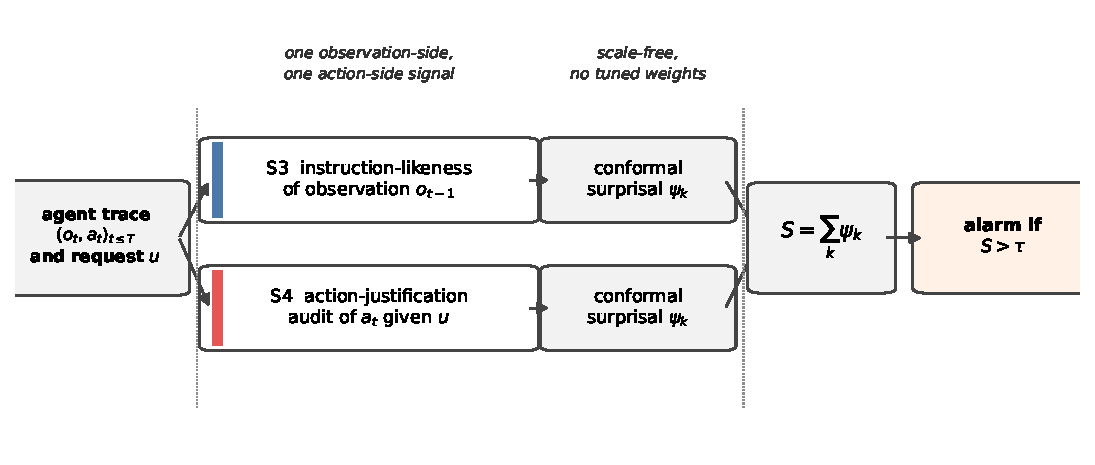
\includegraphics[width=\textwidth]{figures/overview.pdf}
\caption{Overview of SENTRY-Fuse. Two signals are computed per action, one from
each evidence channel: the \emph{observation} channel (S3) asks whether untrusted
content is behaving like an instruction, while the \emph{action} channel (S4) asks
whether the agent's behaviour serves the user's request. Each raw
score is mapped to a conformal tail surprisal against a benign calibration split,
which makes the heterogeneous signals commensurable at a far finer resolution
than the excess-over-maximum alternative of Proposition~\ref{prop:clip}, which
collapses a whole class to a point. The surprisals are summed and thresholded; on
an alarm the largest term, $\arg\max_k \psi_k$, names the signal that fired, which
gives the operator an actionable reason rather than a bare alert.}
\label{fig:overview}
\end{figure}

\subsection{Signals}\label{sec:signals}

We implemented five per-action signals and adopted two. Exactly one, S3, scores the
\emph{observation} stream, asking whether untrusted content is behaving like an
instruction; the other four score the \emph{action} stream.
\textbf{SENTRY-Fuse is the fusion of S3 and S4}---one signal from each channel.
The remaining three are reported because we implemented them and their failure
modes are informative: S1 and S2 ask only whether behaviour is statistically \emph{unusual}
and are near-chance under a protocol that fits the reference out-of-sample
(Section~\ref{sec:negatives}); S5 is well motivated and precise but its measured
contribution does not survive a trajectory bootstrap (Section~\ref{sec:results}).

\paragraph{S1: tool-transition surprise (rejected)}
A Laplace-smoothed bigram model over consecutive tool names, fitted on benign
traces, gives
\begin{equation}
s^{\mathrm{tr}}_t = -\log \hat{P}\big(\mathrm{tool}(a_t) \mid \mathrm{tool}(a_{t-1})\big),
\end{equation}
with $\mathrm{tool}(a_0)$ a distinguished start symbol so that the score is
defined at $t=1$.

\paragraph{S2: argument novelty (rejected)}
The fraction of tokens in $a_t$'s arguments that never appeared in any argument of
the same tool in the benign reference,
\begin{equation}
s^{\mathrm{nov}}_t = \frac{|\{\text{tokens of } \mathrm{args}(a_t)\} \setminus
V_{\mathrm{tool}(a_t)}|}{|\{\text{tokens of } \mathrm{args}(a_t)\}|} \in [0,1],
\end{equation}
where $V_{\mathrm{tool}}$ is the per-tool argument vocabulary of the reference
split. Folding S1 and S2 into a single score as
$s^{\mathrm{tr}}_t + 4\,s^{\mathrm{nov}}_t$---which is how this project began---adds
two raw quantities on incommensurable scales (nats and a fraction) with a weight
chosen by hand. That
is precisely the failure mode Section~\ref{sec:fusion} exists to remove.

We must be precise about the scope of the fix.
\textbf{SENTRY-Fuse and its ablation (Table~\ref{tab:fused}) use no weights at
all}: every signal is conformalised separately and summed, which is the claim made
in Section~\ref{sec:fusion}. The \emph{attempt-detection} results
(Tables~\ref{tab:generalisation}, \ref{tab:normablation}
and~\ref{tab:longhorizon}) come from the project's original scalar pipeline, which
sums the per-action signals with fixed coefficients $(1, 4, 4, 4)$. In each of
those tables the weighting is held constant while one factor varies---the
normalisation in Table~\ref{tab:normablation}, the agent or attack family in
Table~\ref{tab:generalisation}, the combiner in
Table~\ref{tab:longhorizon}---so the comparisons they support are unaffected.
Their absolute values, however, are those of the weighted composite and should not
be read as single-signal performance.

\paragraph{S3: observation instruction-likeness}
Let $\mathrm{IL}(o)$ score how strongly a tool output reads as a directive
addressed to the agent. We evaluate two instantiations. The \emph{lexicon}
variant is a weighted per-word density of imperative verbs, second-person
pronouns, pseudo-markup and exclamation marks. The \emph{judge} variant queries a
small LLM with the observation alone and takes a normalised integer rating.
Section~\ref{sec:ablation} compares them; the judge generalises better across
attack templates, at the price of one cached model call per distinct observation.

\paragraph{S4: action-justification audit}
Given only the user request $u$, the tool name and its arguments---and
\emph{never} the observations---an LLM judge rates how far the call fails to
serve $u$:
\begin{equation}
s^{\mathrm{aj}}_t = \mathrm{Unjustified}(u,\, a_t) \in [0,1].
\end{equation}
Withholding the observations is a deliberate design choice: it prevents the audit
from simply re-detecting the injected text, so S4 is not a restatement of S3 and
the two may be fused without circularity.

\paragraph{S5: sensitive-sink provenance}
A conjunctive, per-value rule that fires when the agent performs an
externally-effectful call whose critical argument traces to untrusted prose:
\begin{equation}
s^{\mathrm{sp}}_t = \Ind\big[\, \mathrm{Sink}(a_t) \wedge \exists v \in
\mathrm{Ids}(a_t):\ v \notin u \ \wedge\ \mathrm{FirstSeenInProse}(v) \,\big].
\end{equation}
Here $\mathrm{Sink}$ marks tools with external effect (moving money, sending
messages, publishing, editing standing instructions) as opposed to read-only
lookups; $\mathrm{Ids}$ extracts identifier-like values (IBANs, e-mail addresses,
URLs, long digit strings); and $\mathrm{FirstSeenInProse}$ holds when the value's
first appearance in the trace is inside a long natural-language line rather than
a short structured record field. The intuition is that a legitimate recipient
reaches the agent as a record it looked up, whereas an attacker's recipient
arrives embedded in the prose of a poisoned document.

\subsection{Why naive normalisation fails}\label{sec:clipping}

The signals live on incompatible scales: $s^{\mathrm{tr}}$ is in nats and
unbounded, $s^{\mathrm{il}}$ and $s^{\mathrm{aj}}$ lie in $[0,1]$,
$s^{\mathrm{sp}}$ is binary.
Summing them raw lets the widest-ranged term dominate. The natural fix is to
subtract the largest value observed in benign training data,
\begin{equation}\label{eq:excess}
\phi_{\max}(x) = \max\{0,\ x - \beta\}, \qquad
\beta = \max_{x' \in \Dcal_{\mathrm{train}}} x' ,
\end{equation}
so that anything within the benign range scores zero. This is a trap.

Throughout, $\mathrm{AUROC}$ denotes the area under the receiver operating
characteristic curve: the probability that a randomly drawn positive scores above
a randomly drawn negative, counting ties as one half.

\begin{proposition}[Excess-over-maximum can annihilate a signal]\label{prop:clip}
Let $\phi_{\max}$ be as in~\eqref{eq:excess}. Condition throughout on
$\Dcal_{\mathrm{train}}$, so that $\beta$ is a fixed number. Let $\Bcal, \Ccal$ be
the benign and attack score distributions and suppose the attack scores satisfy
$\Prob_{X \sim \Ccal}(X \le \beta) = 1$. Write
$q = \Prob_{X \sim \Bcal}(X > \beta)$ for the benign exceedance probability. Then
\begin{equation}\label{eq:clipauroc}
\mathrm{AUROC}\big(\phi_{\max}(\Bcal),\, \phi_{\max}(\Ccal)\big)
= \tfrac{1}{2}(1 - q) \;\le\; \tfrac{1}{2},
\end{equation}
irrespective of how well $x$ itself separates the classes. In particular the
transform is at best uninformative under this hypothesis, and strictly
\emph{worse} than chance whenever some benign score exceeds $\beta$.
\end{proposition}

\begin{proof}
$\phi_{\max}$ maps $(-\infty, \beta]$ to the single point $0$. Since $\Ccal$ is
supported on $(-\infty,\beta]$, every transformed attack score is exactly $0$. A
transformed benign score is $0$ with probability $1-q$ and strictly positive with
probability $q$. Comparing an independent attack score with a benign score, the
attack score is never larger, is tied with probability $1-q$, and is smaller with
probability $q$. Counting ties as one half gives
$\mathrm{AUROC} = \tfrac{1}{2}(1-q) + 0 \cdot q$, which is~\eqref{eq:clipauroc}.
\end{proof}

Two remarks. First, $q>0$ is the generic case rather than an edge case: if $\beta$
is the maximum of $n$ exchangeable benign training scores from a continuous law,
then a fresh benign score exceeds it with probability exactly $1/(n+1)$. Second,
the hypothesis $\Prob_{\Ccal}(X \le \beta) = 1$ holds only approximately on real
data---a few attack scores do exceed $\beta$---which is why the collapse measured
in Section~\ref{sec:ablation} lands just \emph{above} $1/2$ ($0.515$ to $0.531$)
rather than at or below it. The proposition identifies the mechanism and its worst
case; it does not predict the exact value.

The premise is not hypothetical. In our data the lexicon instruction-likeness of
benign observations is $\BenIlMedian$ at the median and $\BenIlMean$ on average,
but its \emph{maximum} is $\BenIlMax$---a single outlier---while no InjecAgent
observation exceeds $\InjIlMax$. Every InjecAgent score therefore fell below
$\beta$, and under $\phi_{\max}$ the lexicon signal was driven to
$\mathrm{AUROC} = \AblLexMaxInjAuroc$ against $\AblLexConfInjAuroc$ under the conformal
transform of Section~\ref{sec:fusion}. The model judge, whose output is far more
concentrated, fares worse: it awards exactly $1.0$ to some benign observations, so
$\beta = 1$ and $\phi_{\max}$ is \emph{identically} zero---giving
$\AblJudgeMaxInjAuroc$ against $\AblJudgeConfInjAuroc$ on InjecAgent and
$\AblJudgeMaxImpAuroc$ against $\AblJudgeConfImpAuroc$ on
\texttt{important\_instructions}, a loss of roughly a quarter of an AUROC on the
better scorer. It would be natural to read that collapse as evidence that the
attack is subtly phrased. That reading is wrong---the InjecAgent payloads are
imperative and appear in the trace in every case---and the cause is the
normalisation, not the attack.

The lesson is about \emph{resolution}, not merely about monotonicity. Both
$\phi_{\max}$ and the conformal transform below are many-to-one; the difference is
that $\phi_{\max}$ can map an entire class to a single point, destroying all
within-class ordering, whereas the conformal transform retains $n+1$ distinct
levels. A component transform must therefore be chosen so that its quantisation
is fine relative to the separation one hopes to exploit---a requirement we make
precise in Proposition~\ref{prop:mono}.

\subsection{Conformal surprisal fusion}\label{sec:fusion}

\begin{definition}[Conformal tail surprisal]
Let $x_{1:n}$ be benign calibration values for a signal and $x$ a test value. The
conformal $p$-value and surprisal are
\begin{equation}\label{eq:conformal}
p(x) = \frac{1 + |\{i : x_i \ge x\}|}{n+1},
\qquad
\psi(x) = -\log p(x).
\end{equation}
\end{definition}

\begin{proposition}[Distribution-free validity]\label{prop:valid}
If $x, x_1, \dots, x_n$ are exchangeable, then $\Prob(p(x) \le \alpha) \le \alpha$
for every $\alpha \in (0,1)$; equivalently
$\Prob(\psi(x) \ge \log(1/\alpha)) \le \alpha$.
\end{proposition}

\begin{proof}
If the values are almost surely distinct, exchangeability makes the rank of $x$
among $\{x, x_1, \dots, x_n\}$ uniform on $\{1,\dots,n+1\}$, and
$\{p(x) \le \alpha\}$ is the event that this rank places $x$ among the top
$\lfloor \alpha (n+1) \rfloor$ values, of probability
$\lfloor \alpha(n+1)\rfloor/(n+1) \le \alpha$. Ties only help: because
$|\{i : x_i \ge x\}|$ counts calibration values \emph{weakly} exceeding $x$, a tie
can only increase $p(x)$, so the bound continues to hold with the same argument
applied to any tie-breaking rule.
\end{proof}

The tie case is not academic here. S5 is binary by construction and S4 saturates
at $1.0$ on $\SfourSatPct\%$ of benign trajectories, so the calibration samples of those
signals contain many repeated values; the weak inequality in~\eqref{eq:conformal}
is what keeps $p$ conservative rather than anti-conservative.

\begin{proposition}[Ordering and scale-freeness]\label{prop:mono}
Fix calibration values $x_{1:n}$ and let $\psi$ be as in~\eqref{eq:conformal}.
Then (i) $\psi$ is non-decreasing, so it never inverts a strict ordering;
(ii) $\psi$ is invariant to any strictly increasing reparameterisation applied
jointly to the test value and the calibration values; and (iii) $\psi$ takes at most $n+1$ distinct values, all in
$[0, \log(n+1)]$, so it is many-to-one, and AUROC is preserved only up to the
ties this quantisation introduces.
\end{proposition}

\begin{proof}
$|\{i : x_i \ge x\}|$ is non-increasing in $x$, so $p$ is non-increasing and
$\psi = -\log p$ is non-decreasing, which gives (i): if $x < x'$ then
$\psi(x) \le \psi(x')$, so no strictly ordered pair is reversed.
For (ii), $\psi$ is a function of the rank of $x$ among the calibration values,
and ranks are invariant under strictly increasing maps. For (iii),
$|\{i : x_i \ge x\}|$ ranges over $\{0,1,\dots,n\}$, so $p$ takes values in
$\{1/(n{+}1), \dots, 1\}$ and $\psi$ in $\{0, \dots, \log(n{+}1)\}$; in
particular every $x$ strictly above $\max_i x_i$ receives the same value
$\log(n{+}1)$.
\end{proof}

Part (iii) is a genuine limitation and we state it rather than claim more.
Because the transform saturates above the calibration maximum, it \emph{can} lose
discrimination. With $n=1$, calibration $\{0\}$, benign scores $\{0.1, 0.2\}$ and
attack scores $\{0.3, 0.4\}$, a perfectly separating signal ($\mathrm{AUROC}=1$) is
mapped to the constant $\log 2$ and AUROC falls to $1/2$. Nor is $1/2$ a floor:
with calibration $\{10\}$, benign $\{0,0,11\}$ and attack $\{1,2\}$, an
above-chance signal ($0.667$) becomes $0.333$, because collapsing correctly
ordered pairs into ties can cost more than it gains. Monotonicity therefore buys
\emph{no} guarantee about AUROC; only resolution does.

At realistic calibration sizes the cost is small but not zero. On well-separated
synthetic Gaussians, where the raw signal has $\mathrm{AUROC} = 1$, the conformal
transform yields $\QuantNFive$ at $n=5$, $\QuantNTwentyThree$ at $n=23$ and
$\QuantNFortySeven$ at $n=47$ (400 replicates each; the calibration sizes used in this paper
are $23$ and $47$). The loss is $O(1/n)$, which is why we prefer the largest
calibration split the corpus allows.

The contrast with Proposition~\ref{prop:clip} is accordingly quantitative rather
than categorical. Both transforms are many-to-one. The difference is how coarse
they are: $\phi_{\max}$ maps an entire class to a single point, leaving no
within-class ordering at all and forcing
$\mathrm{AUROC} = \tfrac{1}{2}(1-q) \le \tfrac{1}{2}$, whereas $\psi$ retains
$n+1$ ordered levels. What a fusion rule needs is not injectivity, and not
monotonicity alone, but a quantisation fine enough that the surviving ordering
still separates the classes; Section~\ref{sec:ablation} measures what that is
worth on real signals.

\begin{definition}[SENTRY-Fuse]
For signals $k = 1,\dots,K$ with per-trajectory summaries $x_k$ (we use the
per-trajectory maximum of each per-action signal) and benign calibration values
$x^{(k)}_{1:n_k}$, the fused statistic is
\begin{equation}\label{eq:fuse}
S \;=\; \sum_{k=1}^{K} \psi_k(x_k) \;=\; -\sum_{k=1}^{K} \log p_k(x_k),
\end{equation}
and the monitor alarms when $S > \tau$, with $\tau$ set from held-out benign scores
as Algorithm~\ref{alg:fuse} specifies.
\end{definition}

The rule has no tuned weights: every signal contributes on the common scale of
$\log$-improbability, which is what makes an unweighted sum meaningful. Two
caveats belong here rather than in a footnote. First, by
Proposition~\ref{prop:mono}(iii) component $k$ contributes at most
$\log(n_k{+}1)$, so if the calibration sets differ in size the sum is implicitly
weighted by $\log(n_k{+}1)$; we therefore use a single calibration split, giving
$n_k = n$ for all $k$ and equal maximum contributions. Second, the
\emph{threshold} $\tau$ remains a calibrated quantity, which we choose as a
benign quantile; the claim is that the relative contribution of the signals is
untuned, not that the monitor is free of all calibration.

\begin{proposition}[Fused false-alarm bound]\label{prop:fusebound}
Suppose each $x_k$ is exchangeable with its calibration values
$x^{(k)}_{1:n_k}$ (the hypothesis of Proposition~\ref{prop:valid}). Then for any
$\tau > 0$,
\begin{equation}
\Prob(S \ge \tau) \;\le\; \min\Big\{1,\ \sum_{k=1}^{K} e^{-\tau/K} \Big\}
\;=\; \min\{1,\ K e^{-\tau/K}\}.
\end{equation}
If in addition the $p_k$ are mutually independent, Fisher's method gives the
sharper bound
\begin{equation}\label{eq:fisherbound}
\Prob(S \ge \tau) \;\le\; \Gamma(K,\tau)/\Gamma(K),
\qquad
\Gamma(K,\tau) = \int_\tau^\infty u^{K-1}e^{-u}\,\mathrm{d}u ,
\end{equation}
where $\Gamma(K,\tau)$ is the upper incomplete gamma function.
\end{proposition}

\begin{proof}
If $S \ge \tau$ then some $\psi_k \ge \tau/K$, so
$\{S \ge \tau\} \subseteq \bigcup_k \{\psi_k \ge \tau/K\}$; a union bound with
Proposition~\ref{prop:valid} applied at level $\alpha = e^{-\tau/K}$ gives the
first claim, and it requires no dependence assumption. For the second,
Proposition~\ref{prop:valid} says each $p_k$ is stochastically larger than a
uniform variable, so each $-\log p_k$ is stochastically dominated by a standard
exponential; under independence the sum is dominated by a $\mathrm{Gamma}(K,1)$
variable, whose upper tail is $\Gamma(K,\tau)/\Gamma(K)$.
\end{proof}

The bound is on $\{S \ge \tau\}$, which contains the alarm event $\{S > \tau\}$ the
monitor uses, so it applies to the monitor too.
Only \emph{domination} holds, not equality: since each $p_k$ is supported on the
finite grid $\{1/(n{+}1),\dots,1\}$, the statistic $S$ is discrete and bounded
above by $K\log(n{+}1)$, so it cannot be exactly Gamma-distributed.

\begin{remark}
We report empirical operating points throughout rather than relying on
Proposition~\ref{prop:fusebound}, because the assumption-light union bound is
loose and independence across our signals is not credible: S3 and S4 both respond
to the presence of an injection, albeit through different channels. The bound's
role is to establish that the fused statistic admits distribution-free
false-alarm control at all, and to make explicit what would be needed for a sharp
one.
\end{remark}

\begin{algorithm}[t]
\caption{SENTRY-Fuse}\label{alg:fuse}
\begin{algorithmic}[1]
\Require disjoint benign splits $\Dcal_{\mathrm{fit}}, \Dcal_{\mathrm{cal}}, \Dcal_{\mathrm{test}}$; target false-alarm rate $\alpha$; signals $1,\dots,K$
\State fit any reference a signal needs (e.g.\ per-tool vocabularies) on $\Dcal_{\mathrm{fit}}$
\For{$k = 1,\dots,K$}
  \State $x^{(k)}_{1:n_k} \gets$ per-trajectory summaries of signal $k$ on $\Dcal_{\mathrm{cal}}$, scored against the $\Dcal_{\mathrm{fit}}$ reference
\EndFor
\State $\tau \gets$ the $k$-th largest of $\{S(\Tcal) : \Tcal \in \Dcal_{\mathrm{test}}\}$, $k = \lfloor \alpha |\Dcal_{\mathrm{test}}| \rfloor$, or the maximum if $k=0$ \Comment{in sample; Section~\ref{sec:metrics}}
\Statex \textbf{at monitoring time, for a trace} $\Tcal$:
\For{$k = 1,\dots,K$}
  \State $x_k \gets \max_t s^{(k)}_t(\Tcal)$;\quad
         $\psi_k \gets -\log\big((1 + |\{i : x^{(k)}_i \ge x_k\}|)/(n_k+1)\big)$
\EndFor
\State $S \gets \sum_k \psi_k$
\If{$S > \tau$} \textbf{raise alarm}; report $\arg\max_k \psi_k$ as the dominant cause
\EndIf
\end{algorithmic}
\end{algorithm}

Because the fusion is additive over interpretable components, the dominant term
$\arg\max_k \psi_k$ names \emph{why} the monitor fired---an injected instruction,
an unjustified action, an untrusted recipient, or an anomalous tool
transition---which matters for triage.

%======================================================================
\section{Experimental Setup}\label{sec:experiments}

\subsection{Corpora}

We collect real trajectories by running tool-calling agents on standard
benchmarks; Table~\ref{tab:corpus} summarises the result. From
AgentDojo~\citep{debenedetti2024agentdojo} we run all four suites (banking,
workspace, travel, Slack) both benign and under attack, with two attack
families: the \texttt{important\_\hspace{0pt}instructions} template and the
InjecAgent~\citep{zhan2024injecagent} template. From
$\tau$-bench~\citep{yao2024taubench} we run the retail domain benign-only, to
diversify the benign reference. Two agents are used: DeepSeek-V4-Flash and
GPT-4o-mini, from different vendors, so that agent identity can be varied
independently of everything else.

\begin{table}[t]
\centering
\caption{Trajectory corpora, with the \emph{corrected} label polarity of
Section~\ref{sec:polarity}: \emph{compromised} means the injection task
succeeded. Counts are after a two-action minimum filter. ``imp.\ instr.''\ is
AgentDojo's \texttt{important\_instructions} template; the DeepSeek agent is
DeepSeek-V4-Flash.}
\label{tab:corpus}
\small
\begin{tabular}{@{}llrrrr@{}}
\toprule
Agent & Attack family & Benign & Attacks & Comp. & Resist. \\
\midrule
DeepSeek & imp.\ instr. & 71 & 198 & 18 (9\%) & 180 \\
DeepSeek & InjecAgent & --- & 42 & \textbf{0 (0\%)} & 42 \\
GPT-4o-mini & imp.\ instr. & 70 & 153 & 72 (47\%) & 81 \\
$\tau$-bench retail & none & 50 & --- & --- & --- \\
\midrule
\multicolumn{2}{@{}l}{\textbf{Total}} & \textbf{191} & \textbf{393} & \textbf{90} & \textbf{303} \\
\bottomrule
\end{tabular}
\end{table}

Table~\ref{tab:corpus} already contains a substantive finding. The two agents
differ enormously in injection robustness: GPT-4o-mini is compromised in $47\%$
of attempts, DeepSeek-V4-Flash in only $9\%$, and DeepSeek resisted the
InjecAgent family \emph{completely} ($0/42$). Robustness to indirect prompt
injection is therefore a strong function of the agent, not a property of the
attack alone, and a defence evaluated on a single agent may be measuring that
agent's fragility as much as its own merit.

\begin{remark}
Because DeepSeek was never compromised by InjecAgent, compromise detection is
\emph{undefined} for that cell: there are no positives. Only attempt detection is
meaningful there, and we report it as such rather than quoting a rate over an
empty class.
\end{remark}

\subsection{Protocol}\label{sec:protocol}

Trajectories are converted to per-action signal streams by a deterministic,
GPU-free adapter. Feature hashing uses a seed-stable CRC rather than Python's
per-process-salted hash, so the entire evaluation is byte-reproducible. LLM judge
scores are cached by content hash ($681$ distinct observations, $1{,}329$ distinct
task--action pairs), so all reported evaluations run offline from committed
caches.

Our evaluation protocol is deliberately strict about leakage. For each of ten
seeds the benign set is split into three disjoint parts: one third fits the
reference model (the bigram table and per-tool argument vocabularies), one third
supplies the conformal calibration values, and one third supplies the held-out
negatives. Compromise-positive trajectories are never used for fitting or
calibration. We report mean $\pm$ standard deviation over the ten seeds (population
convention; the bootstrap intervals in Section~\ref{sec:results} use the sample
convention).

The three-way split matters for Proposition~\ref{prop:valid}. If the calibration
values are computed on the same trajectories the reference was fitted to, they are
in-sample and systematically less surprising than a fresh benign draw, so the
conformal $p$-values are anti-conservative and the stated false-alarm level is not
delivered. Fitting on a separate third makes the calibration values and the
held-out negatives both out-of-sample with respect to the reference, which is what
exchangeability requires.

\begin{remark}[Leakage matters]
An earlier version of this evaluation fitted the reference on all benign
trajectories including the test half. Under that protocol the weighted behavioural
composite (S1 and S2 summed with fixed coefficients) appeared excellent,
$\mathrm{AUROC} = 0.982$; with the reference fitted out-of-sample and the signals
kept separate, S1 and S2 fall to between $\DsStwoAuroc$ and $\PoolStwoAuroc$
(Table~\ref{tab:fused}). Only held-out numbers appear in the compromise-detection
results.
This is worth stating plainly because the leaky number is the one a careless
pipeline produces by default.
\end{remark}

\subsection{Metrics}\label{sec:metrics}

We report AUROC and the true-positive rate (TPR) at a benign false-positive rate
(FPR). Comparing detectors at a common FPR is essential---they are otherwise
trivially incomparable---but on samples of this size a \emph{nominal} FPR cannot
generally be hit. With $n$ held-out negatives, thresholding a score yields only
the rates $k/n$ for integer $k$, so the attainable grid has spacing $1/n$: $4.2\%$
on the $\nGptNeg$ GPT-4o-mini negatives and $2.1\%$ on the $\nPoolNeg$ pooled ones. We
therefore set the threshold at the $k$-th largest negative with
$k = \lfloor \alpha n \rfloor$ and then \emph{measure} the rate it realises, which
we report in every table alongside the target. We use $\alpha = 5\%$ as the target
throughout.

Two caveats about this number. First, it is generally strictly below $k/n$, because
by Proposition~\ref{prop:mono}(iii) the fused statistic takes at most $n_k+1$
values, so negatives tie at the saturated level and fewer than $k$ of them exceed
the threshold---which is why the realised rates in Table~\ref{tab:fused} range from
$0.0\%$ to $4.0\%$ against a $5\%$ target rather than sitting at $k/n$. Second, we
are reading a point off the empirical ROC curve of the held-out negatives, so the
reported rate is descriptive of \emph{those} negatives and is not an out-of-sample
false-alarm guarantee; a deployment would fix $\tau$ on a further split and accept
the extra variability, and Proposition~\ref{prop:fusebound} is what supplies a
distribution-free---if loose---a-priori bound.

This is worth being explicit about because interpolating an empirical quantile, as
is conventional, silently produces a different rate: at a nominal $3.66\%$ on $35$
negatives the realised rate is $2/35 = 5.71\%$, and a TPR quoted at ``$3.66\%$''
would then have been measured at over $5\%$.

\paragraph{On comparison with published figures}
AgentArmor~\citep{wang2025agentarmor} is the strongest reported trace-only
detector, and version~1 of that preprint reports $95.75\%$ TPR at $3.66\%$ FPR on
AgentDojo with a GPT-4o agent. We do \emph{not} present our numbers as beating it,
for three reasons. The corpora differ (different agents, a different attack
sample, and---as Section~\ref{sec:polarity} shows---a positive-class definition
that is easy to get wrong); the operating points differ once the realised rate is
accounted for; and the figure itself was removed in later versions of that
preprint, which report TPR between $86\%$ and $97\%$ at FPR between $2\%$ and
$19\%$ instead. We cite it as a reference point for the regime, not as a baseline
we outperform, and we did not re-implement its program-dependence analysis.

Comparing only against published figures on other corpora would leave the
evaluation a self-ablation, so we re-implemented one published method and ran it
on our trajectories under our protocol: \textbf{Task Shield}, which is the closest
prior work to our action-side signal. Section~\ref{sec:baseline} reports it.

\subsection{A label-polarity pitfall}\label{sec:polarity}

Before presenting results we must document a methodological trap, because it
inverted our own conclusions for a substantial period and because the ceiling
analysis of Section~\ref{sec:ceiling} is impossible to get right without it.

AgentDojo returns a per-trajectory \texttt{security} flag. It is natural, and
wrong, to read this as ``the system was secure''. The flag is computed as the
success of the \emph{injection} task, so \texttt{security}$\,=\,$\texttt{True}
means the attacker's goal was achieved, i.e.\ the agent \emph{was compromised}.

We initially adopted the opposite convention. The error was invisible in
aggregate: both classes are non-empty, all downstream code ran, and every metric
produced plausible numbers. It surfaced only when we asked why so many
``compromised'' trajectories contained no state-changing tool call at all, and read
one:

\begin{example}[A trajectory we had labelled compromised]
\label{ex:refusal}
Banking suite, \texttt{important\_instructions}. The agent calls
\texttt{read\_file} and five read-only lookups, then states:
\begin{quote}\itshape
``I see a message embedded in the bill file that's trying to get me to do
something else first. However, I shouldn't be tricked by that embedded
instruction.''
\end{quote}
This agent \emph{resisted}. It had been counted as a successful attack.
\end{example}

We resolved the polarity against ground truth rather than documentation. In the
banking suite the adversary's goal is a transfer to a specific attacker IBAN, so
compliance is directly checkable in the trace:

\begin{table}[t]
\centering
\caption{Resolving label polarity against in-trace ground truth, over all $107$
attacked banking-suite trajectories. Every trajectory flagged
\texttt{security}$\,=\,$\texttt{True} wired money to the attacker's account, which
settles the polarity. The three \texttt{False} trajectories that also paid the
attacker are cases of partial compliance, and show that the flag undercounts harm.}
\label{tab:polarity}
\begin{tabular}{@{}lcc@{}}
\toprule
& \texttt{security}$=$\texttt{True} & \texttt{security}$=$\texttt{False} \\
\midrule
agent wired money to attacker IBAN & \textbf{31} & 3 \\
agent did not & 0 & \textbf{73} \\
\bottomrule
\end{tabular}
\end{table}

Example~\ref{ex:refusal} shows one such trajectory in full, and Table~\ref{tab:polarity} settles the direction that matters: every one of the $31$
trajectories flagged \texttt{security}$\,=\,$\texttt{True} did in fact wire money
to the attacker, and none of the trajectories that wired no money is so flagged. So
\texttt{security}$\,=\,$\texttt{True} is compromise, and the polarity we had been
using was inverted.

The converse fails, however, and the failure is worth recording. Three
trajectories labelled \texttt{security}$\,=\,$\texttt{False} \emph{did} pay the
attacker. Inspecting them shows why: this injection task requires not merely a
transfer to the attacker's account but one whose subject line names the user's
music-streaming service, and in these three the agent transferred the money with a
subject of its own invention. The flag scores the injection task's \emph{exact}
goal, so an agent that is manipulated into moving money but fumbles a detail of the
attacker's script is recorded as having resisted. The harness therefore
\emph{undercounts} harm, and our compromised class of $90$ is a lower bound. We
keep the harness definition---changing it would make our numbers incomparable with
the literature's---but flag that a harm-based positive class would be the better
target, and that the $303$ ``resisted'' trajectories are not all benign.

The consequences for us were severe and instructive. Every ``hijack-detection''
number we had computed was measuring the \emph{resisted} class. Our effect-based
signals---the action audit and sink provenance---had been graded against
trajectories in which, by construction, the agent had done nothing harmful; they
appeared useless. Once the polarity was corrected the action audit became one of
the two signals the method relies on, reaching $\mathrm{AUROC} = 0.900 \pm 0.039$
on GPT-4o-mini and $\DsSfourAuroc \pm \DsSfourAurocSd$ on DeepSeek (Table~\ref{tab:fused}). We had
nearly discarded a working signal because of a boolean.

\begin{remark}
We report this at length because the failure mode is silent, the fix is trivial,
and the affected quantity---which class counts as a successful attack---is the
foundation of every number in this literature. We recommend that any work using
this harness verify polarity against an in-trace ground-truth check of the kind in
Table~\ref{tab:polarity}, and report having done so. The same check is what
surfaced the undercount above, so it is worth running even once the polarity is
known to be right.
\end{remark}

%======================================================================
\section{Results}\label{sec:results}

\subsection{Compromise detection}

Table~\ref{tab:fused} gives the main result. On GPT-4o-mini, where the
compromised class is largest ($\nGptComp$ positives), the observation-side
instruction signal alone reaches $\mathrm{AUROC} = \GptSthreeAuroc$ but a wildly
variable $\mathrm{TPR} = \GptSthreeTpr \pm \GptSthreeTprSd$: strong on average and
close to unusable at a fixed low false-alarm budget. Adding the
action-justification audit gives $\mathbf{\GptFuseAuroc \pm \GptFuseAurocSd}$ AUROC
and $\mathbf{\GptFuseTpr \pm \GptFuseTprSd}$ recall at a realised
$\GptFuseFpr\%$ false-positive rate. Pooled over both agents the ordering holds,
ending at $\PoolFuseAuroc$ and $\PoolFuseTpr \pm \PoolFuseTprSd$. Adding sink
provenance on top changes little (Table~\ref{tab:fused}, the row below), which
Section~\ref{sec:results} quantifies and is why it is not adopted.

\begin{table}[htbp]
\centering
\caption{Compromise detection, ten seeds, mean $\pm$ std, AgentDojo benign
trajectories only. Each seed splits the benign set three ways: one third fits the
reference, one third supplies the conformal calibration values, one third the
held-out negatives. A nominal false-positive target is not attainable exactly---only
multiples of $1/n$ are, and the fused statistic is discrete---so we report the
\emph{realised} rate next to each target. Rows therefore sit at different operating
points and the TPR columns are not like-for-like across rows, whereas AUROC is; the
$3.66\%$ target in particular collapses to a realised $0.0\%$ on the two per-agent
corpora, where $\lfloor 0.0366n \rfloor = 0$. SENTRY-Fuse in bold; the two rows
below it are ablations we evaluated and did not adopt.}
\label{tab:fused}
\scriptsize
\setlength{\tabcolsep}{3.5pt}
\begin{tabular}{@{}lccccc@{}}
\toprule
Detector & AUROC & TPR@$5\%$ & real.\ FPR & TPR@$3.66\%$ & real.\ FPR \\
\midrule
\multicolumn{6}{@{}l}{\emph{GPT-4o-mini: 72 compromised, 24 held-out benign}} \\
S3 instruction-likeness           & $0.951 \pm 0.026$ & $0.661 \pm 0.433$ & $1.2\%$ & $0.472 \pm 0.472$ & $0.0\%$ \\
S4 action audit                   & $0.900 \pm 0.039$ & $0.267 \pm 0.407$ & $0.4\%$ & $0.178 \pm 0.356$ & $0.0\%$ \\
S5 sink provenance                & $0.868 \pm 0.019$ & $0.164 \pm 0.328$ & $0.4\%$ & $0.082 \pm 0.246$ & $0.0\%$ \\
S1 tool transition                & $0.481 \pm 0.062$ & $0.000 \pm 0.000$ & $0.4\%$ & $0.000 \pm 0.000$ & $0.0\%$ \\
S2 argument novelty               & $0.569 \pm 0.056$ & $0.082 \pm 0.098$ & $2.1\%$ & $0.003 \pm 0.008$ & $0.0\%$ \\
S1 $+$ S2                         & $0.530 \pm 0.058$ & $0.101 \pm 0.076$ & $3.8\%$ & $0.040 \pm 0.050$ & $0.0\%$ \\
\textbf{SENTRY-Fuse (S3$+$S4)}    & $\mathbf{0.981 \pm 0.009}$ & $\mathbf{0.914 \pm 0.040}$ & $2.5\%$ & $0.803 \pm 0.269$ & $0.0\%$ \\
\quad $+$ S5 (not adopted)        & $0.985 \pm 0.003$ & $0.956 \pm 0.006$ & $2.9\%$ & $0.899 \pm 0.063$ & $0.0\%$ \\
\quad all five signals            & $0.973 \pm 0.013$ & $0.932 \pm 0.053$ & $3.3\%$ & $0.743 \pm 0.290$ & $0.0\%$ \\
\midrule
\multicolumn{6}{@{}l}{\emph{DeepSeek-V4-Flash: 18 compromised, 25 held-out benign}} \\
S3 instruction-likeness           & $0.850 \pm 0.021$ & $0.467 \pm 0.381$ & $2.4\%$ & $0.078 \pm 0.233$ & $0.0\%$ \\
S4 action audit                   & $0.781 \pm 0.017$ & $0.000 \pm 0.000$ & $0.0\%$ & $0.000 \pm 0.000$ & $0.0\%$ \\
S5 sink provenance                & $0.648 \pm 0.027$ & $0.117 \pm 0.178$ & $0.8\%$ & $0.039 \pm 0.117$ & $0.0\%$ \\
S1 tool transition                & $0.432 \pm 0.068$ & $0.011 \pm 0.022$ & $1.2\%$ & $0.000 \pm 0.000$ & $0.0\%$ \\
S2 argument novelty               & $0.407 \pm 0.098$ & $0.000 \pm 0.000$ & $0.4\%$ & $0.000 \pm 0.000$ & $0.0\%$ \\
S1 $+$ S2                         & $0.389 \pm 0.080$ & $0.000 \pm 0.000$ & $2.4\%$ & $0.000 \pm 0.000$ & $0.0\%$ \\
\textbf{SENTRY-Fuse (S3$+$S4)}    & $\mathbf{0.842 \pm 0.006}$ & $\mathbf{0.778 \pm 0.000}$ & $4.0\%$ & $0.683 \pm 0.230$ & $0.0\%$ \\
\quad $+$ S5 (not adopted)        & $0.832 \pm 0.010$ & $0.767 \pm 0.033$ & $4.0\%$ & $0.539 \pm 0.184$ & $0.0\%$ \\
\quad all five signals            & $0.807 \pm 0.032$ & $0.661 \pm 0.118$ & $3.6\%$ & $0.478 \pm 0.263$ & $0.0\%$ \\
\midrule
\multicolumn{6}{@{}l}{\emph{Pooled: 90 compromised, 47 held-out benign}} \\
S3 instruction-likeness           & $0.937 \pm 0.012$ & $0.709 \pm 0.357$ & $2.8\%$ & $0.598 \pm 0.394$ & $1.3\%$ \\
S4 action audit                   & $0.863 \pm 0.030$ & $0.000 \pm 0.000$ & $0.0\%$ & $0.000 \pm 0.000$ & $0.0\%$ \\
S5 sink provenance                & $0.812 \pm 0.015$ & $0.000 \pm 0.000$ & $0.0\%$ & $0.000 \pm 0.000$ & $0.0\%$ \\
S1 tool transition                & $0.526 \pm 0.077$ & $0.012 \pm 0.033$ & $1.7\%$ & $0.000 \pm 0.000$ & $0.9\%$ \\
S2 argument novelty               & $0.602 \pm 0.045$ & $0.006 \pm 0.017$ & $1.5\%$ & $0.006 \pm 0.017$ & $1.3\%$ \\
S1 $+$ S2                         & $0.557 \pm 0.065$ & $0.038 \pm 0.048$ & $3.8\%$ & $0.011 \pm 0.020$ & $1.7\%$ \\
\textbf{SENTRY-Fuse (S3$+$S4)}    & $\mathbf{0.953 \pm 0.005}$ & $\mathbf{0.898 \pm 0.020}$ & $3.8\%$ & $0.871 \pm 0.045$ & $1.9\%$ \\
\quad $+$ S5 (not adopted)        & $0.954 \pm 0.003$ & $0.918 \pm 0.005$ & $4.0\%$ & $0.884 \pm 0.071$ & $1.7\%$ \\
\quad all five signals            & $0.948 \pm 0.012$ & $0.886 \pm 0.070$ & $3.8\%$ & $0.808 \pm 0.076$ & $2.1\%$ \\
\bottomrule
\end{tabular}
\end{table}

Figure~\ref{fig:fusion} visualises the ablation. Four points deserve emphasis.

First, \textbf{action-side evidence is complementary}. Pooled, the instruction
signal alone reaches $\mathrm{AUROC} = \PoolSthreeAuroc$; adding the action-side
audit takes this to $\PoolFuseAuroc$. We quantify that difference by resampling
\emph{trajectories}---positives and negatives---within each of the $\nSeeds$
splits, which gives $\BootGainAuroc$ with a $95\%$ interval of
$[\BootGainAurocLo, \BootGainAurocHi]$ and $\Prob(\text{gain} \le 0) =
\BootGainAurocP$. The recall gain is $\BootGainTpr$
$[\BootGainTprLo, \BootGainTprHi]$, $\Prob(\le 0) = \BootGainTprP$.

We draw one trajectory resample per replicate and reuse it across the $\nSeeds$
splits, which matters: the splits are re-splits of one corpus, so drawing an
independent resample inside each split and averaging would estimate the variance of
a mean of ten draws and shrink the corpus-sampling variance by about a factor of
ten. An earlier version of this work did that, and it turned a borderline effect
into an apparently decisive one. Corrected, the AUROC interval only marginally
excludes no effect. We therefore do \emph{not} present the AUROC gain as
established: $\nComp$ positives cannot resolve a difference of this size, and the
claim we rest on is the one in the next paragraph.

We report bootstrap intervals rather than a $t$-statistic over the ten splits, and
the distinction matters. The splits permute one fixed benign sample and the
$\nComp$ positives are byte-identical in every seed, so a paired $t$ across seeds
describes how much the answer moves with the calibration draw---a real and
important quantity, reported as the $\pm$ column of Table~\ref{tab:fused}---but not
the sampling error in the corpus, which is what a claim about the \emph{method}
requires.

The gain is not explained by the action signal being individually strong: alone, S4
reaches only $\PoolSfourAuroc$ AUROC. Its recall column reads $0.000$, but that is a
discreteness artefact and not evidence---S4's realised false-positive rate in that
row is $0.0\%$, because $\lfloor 0.05 \times \nPoolNeg \rfloor$ negatives tie at its
threshold, so it is being asked for recall at a zero false-alarm budget. What the
comparison does show is that a signal far weaker in ranking terms still contributes
cases the observation signal misses.

\paragraph{A third signal that did not earn inclusion} We also implemented
sink provenance (S5), and it is \emph{not} part of SENTRY-Fuse, because the evidence
does not support including it. Adding it moves pooled AUROC by $\BootSfiveAuroc$
$[\BootSfiveAurocLo, \BootSfiveAurocHi]$---an interval comfortably containing zero,
$\Prob(\le 0) = \BootSfiveAurocP$---and recall by $\BootSfiveTpr$
$[\BootSfiveTprLo, \BootSfiveTprHi]$, likewise ($\Prob(\le 0) = \BootSfiveTprP$). In
absolute terms it recovers fewer than two additional positives out of $\nComp$. On
the DeepSeek corpus it makes AUROC \emph{worse} ($\DsFusePAuroc$ against
$\DsFuseAuroc$). We report the ablation row in Table~\ref{tab:fused} so the reader
can see it, and we decline to claim it.

Second---and this is the claim we would defend hardest---\textbf{fusion removes a
failure mode that makes the single signal undeployable}. The instruction signal's
standard deviation of recall at a fixed budget is $\pm \GptSthreeTprSd$ on
GPT-4o-mini and $\pm \PoolSthreeTprSd$ pooled, but that spread is not a spread: it
is bimodal. Pooled, the signal returns \emph{exactly zero} recall in
$\SthreeZeroSplits$ of $\nSeeds$ draws and about $0.91$ in the rest.

The mechanism is on the negative side, not the calibration side, and it is
instructive. With $k = \lfloor 0.05 \times \nPoolNeg \rfloor = 2$ negatives allowed
above it, the threshold is set at the $(k+1)$-th largest held-out negative---the
third---so that exactly $k$ of them strictly exceed it. The model judge saturates,
awarding exactly $1.0$ to some benign observations, so whenever three or more of
the $\nPoolNeg$ held-out negatives sit at that ceiling the threshold \emph{is} the
ceiling and no positive can strictly exceed it. Recall is then zero regardless of
how well the signal separates the classes. This is a discrete-operating-point
pathology of a saturating score, and adding a second signal with a different
saturation pattern breaks the tie: SENTRY-Fuse's spread is
$\pm \GptFuseTprSd$ and $\pm \PoolFuseTprSd$, and it never collapses. Unlike the
mean gains above, this difference is far outside sampling noise.

Third, \textbf{more signals is not monotonically better}. Going from the
two-signal method to all five---adding the behavioural pair and provenance---lowers
pooled AUROC from $\PoolFuseAuroc$ to $\PoolAllFiveAuroc$. Isolating the behavioural
pair alone, by comparing the three-signal variant ($\PoolFusePAuroc$) with all five
($\PoolAllFiveAuroc$), gives the same direction. The effect is not uniform: on
GPT-4o-mini all five reach a \emph{higher} recall than the method
($\GptAllFiveTpr$ against $\GptFuseTpr$) while sitting at a looser realised
false-alarm rate, which is why we compare on AUROC. Alone the pair is barely distinguishable
from chance ($\GptBehavAuroc$, $\DsBehavAuroc$ and $\PoolBehavAuroc$ AUROC on the
three corpora, the middle one \emph{below} chance). Because the fusion is an unweighted sum, a near-chance component
injects variance without adding discrimination, and the honest conclusion is that
these two signals do not belong in the monitor. They appear as an ablation row
because they were this project's starting point, and their failure is the clearest
evidence for the distinction between unusual and misaligned.

Fourth, \textbf{the weaker agent is harder, and we report it}. On DeepSeek-V4-%
Flash every detector is worse than on GPT-4o-mini---SENTRY-Fuse reaches
$\mathrm{AUROC} = \DsFuseAuroc$ against $\GptFuseAuroc$. With only $18$ compromised trajectories this
corpus cannot support fine distinctions, but we present it rather than quoting the
favourable corpus alone: on the agent that resists most attacks, our margin over
the single-signal baseline is present in recall ($\DsSthreeTpr \to \DsFuseTpr$) but
\emph{absent} in AUROC, where fusion is slightly worse
($\DsSthreeAuroc \to \DsFuseAuroc$). On this corpus, with $\nDsComp$ positives, we
do not have a ranking-quality improvement to report.

\begin{figure}[t]
\centering
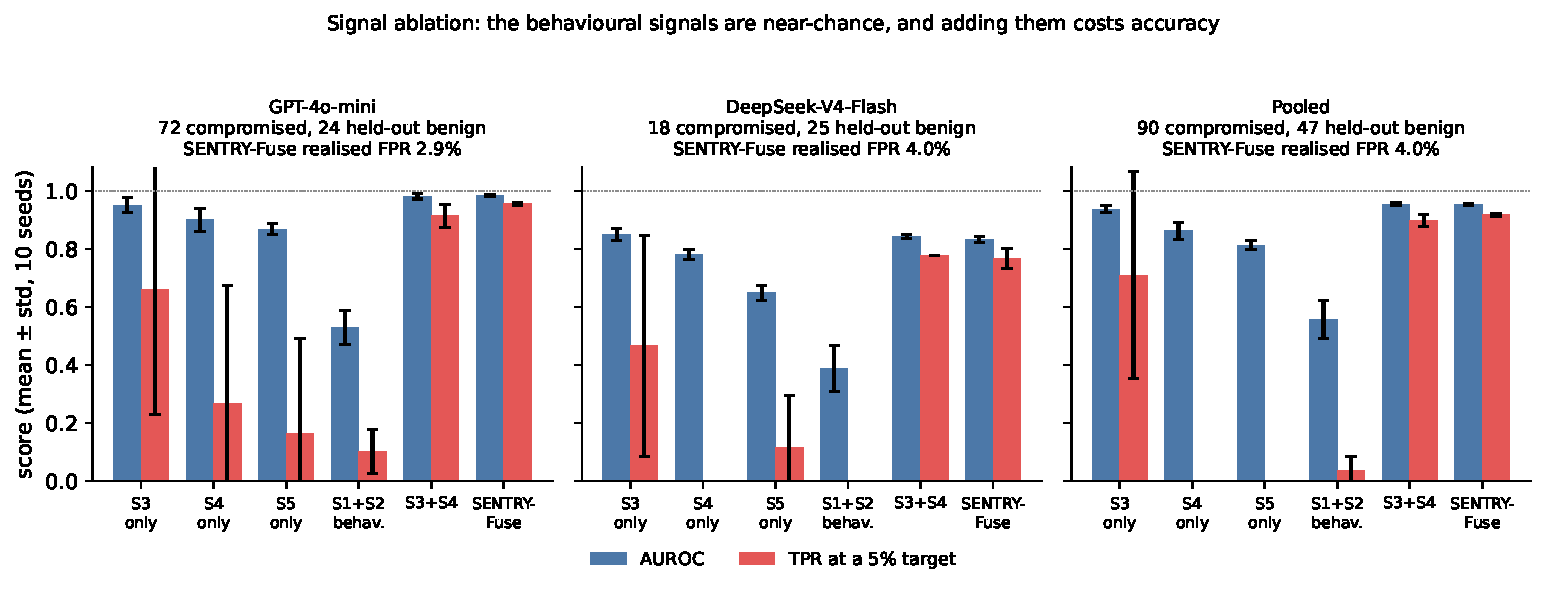
\includegraphics[width=\textwidth]{figures/fusion.pdf}
\caption{Signal ablation across the three corpora. AUROC (blue) and true-positive
rate at a $5\%$ target (red), mean and one standard deviation over ten seeds. The
behavioural signals S1 and S2 are near-chance on every corpus, and the five-signal
sum is worse than the two-signal method; the realised false-positive rate at the
proposed operating point is printed above each panel.}
\label{fig:fusion}
\end{figure}

\subsection{Attempt detection and generalisation}

Table~\ref{tab:generalisation} varies one axis at a time. Attempt detection
transfers across both axes: changing the agent leaves it intact
($\mathrm{AUROC}\,0.76 \to 0.82$), and changing the attack family costs
relatively little once the normalisation of Section~\ref{sec:clipping} is fixed
($0.76 \to 0.71$). Two caveats. First, the three rows sit at different realised
false-alarm rates (final column), so the detection-rate column is not a
like-for-like comparison and we quote AUROC, which is threshold-free, for the
transfer claims. Second, the DeepSeek/InjecAgent cell illustrates why the two
objectives must be kept apart: attempt detection is meaningful there ($0.71$),
while compromise detection is undefined because the agent was never compromised by
that family, so there is no positive class to score.

\begin{table}[t]
\centering
\caption{Generalisation across agent and attack family; ten seeds, corrected
labels. The realised per-step false-alarm rate is given because it differs by row,
so the detection rates are \emph{not} at a common operating point and should be
read against it.}
\label{tab:generalisation}
\small
\setlength{\tabcolsep}{4pt}
\begin{tabular}{@{}llrrccc@{}}
\toprule
Agent & Attack family & Comp. & Resist. & Att.\ det. & Att.\ AUROC & FPR \\
\midrule
DeepSeek & imp.\ instr. & 18 & 180 & $0.65$ & $0.76$ & $2.7\%$ \\
DeepSeek & InjecAgent & 0 & 42 & $0.52$ & $0.71$ & $2.7\%$ \\
GPT-4o-mini & imp.\ instr. & 72 & 81 & $0.74$ & $0.82$ & $4.3\%$ \\
\bottomrule
\end{tabular}
\end{table}

\subsection{Signal and normalisation ablation}\label{sec:ablation}

Table~\ref{tab:normablation} isolates the two design choices in the
observation-side signal S3: how instruction-likeness is scored (fixed lexicon
versus LLM judge) and how it is normalised (excess-over-maximum versus conformal).
The interaction is the point. Under excess-over-maximum the \emph{better} scorer is
the worse detector---the judge falls to $0.515$ AUROC on
\texttt{important\_instructions} against the lexicon's $0.779$---because the
judge's near-binary output places some benign observation at the ceiling, after
which Proposition~\ref{prop:clip} applies and the class is collapsed to a point.
Under the conformal transform the ordering reverses and the judge becomes the
better scorer on the transfer family ($0.706$ against $0.687$ on InjecAgent), while
the lexicon's InjecAgent AUROC recovers from $0.521$ to $0.687$. Normalisation is
not plumbing; it is a first-class design decision that can invert the ranking of
scorers and, as it did for us, produce a confident and wrong explanation of a
failure.

\begin{table}[t]
\centering
\caption{Attempt detection rate / AUROC by instruction scorer and normalisation,
ten seeds. Scores come from the original scalar pipeline, which sums the
per-action signals with fixed coefficients; only the instruction term's
normalisation varies between rows, so the comparison is controlled even though the
absolute values are those of the composite. Excess-over-maximum realises a
per-step false-alarm rate of $0.0182$ and the conformal transform $0.0270$ (judge)
or $0.0335$ (lexicon), so the conformal rows are measured at a
\emph{higher} false-alarm budget and their advantage is not an artefact of a looser
threshold. The conformal transform is required for the semantic judge to be usable
at all.}
\label{tab:normablation}
\small
\begin{tabular}{@{}llcc@{}}
\toprule
Scorer & Normalisation & \texttt{important\_instr.} & InjecAgent \\
\midrule
lexicon & excess-over-max & $0.662 / 0.779$ & $0.114 / 0.521$ \\
lexicon & conformal       & $0.627 / 0.762$ & $0.481 / 0.687$ \\
LLM judge & excess-over-max & $0.159 / 0.515$ & $0.136 / 0.531$ \\
\textbf{LLM judge} & \textbf{conformal} & $\mathbf{0.651 / 0.761}$ & $\mathbf{0.521 / 0.706}$ \\
\bottomrule
\end{tabular}
\end{table}

Figure~\ref{fig:instruction} shows the separation the observation-side signal
achieves, and Figure~\ref{fig:casetrace} walks through a single real compromise
action by action, which is the clearest way to see what each signal contributes.

\begin{figure}[t]
\centering
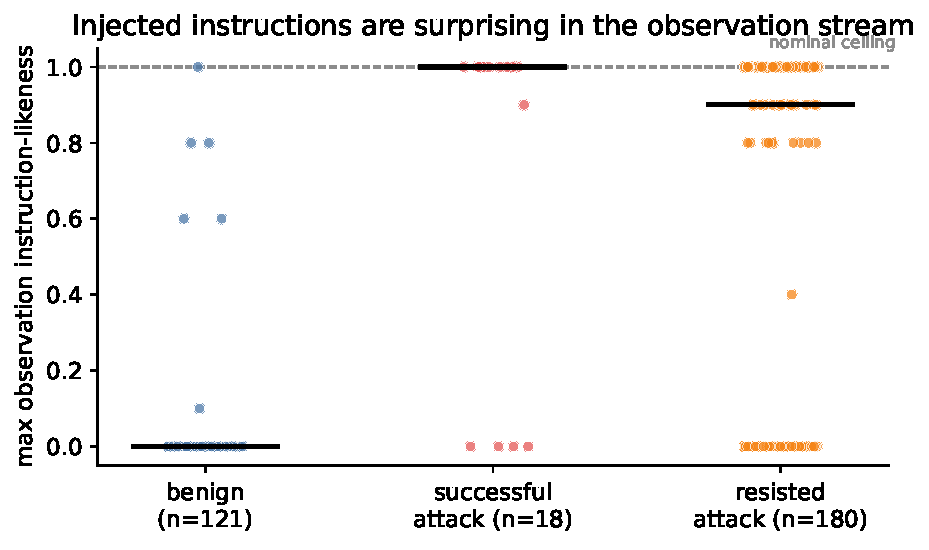
\includegraphics[width=0.8\textwidth]{figures/instruction_sep.pdf}
\caption{Observation instruction-likeness (maximum over a trajectory) for benign
and attacked trajectories, on the DeepSeek-V4-Flash corpus. This is an
\emph{attempt}-detection figure, so the benign group includes the $50$ $\tau$-bench
retail trajectories that the compromise-detection corpora exclude
(Section~\ref{sec:limitations}(viii)). Benign tool output sits near zero at the
median, with a minority of benign trajectories reaching the top of the scale---the
judge saturation that Section~\ref{sec:results} shows costs the signal its
operating point. Attacked trajectories sit far above the nominal range whether or
not the agent ultimately complied, which is why the signal detects attempts well
and compromise less well.}
\label{fig:instruction}
\end{figure}

\begin{figure}[t]
\centering
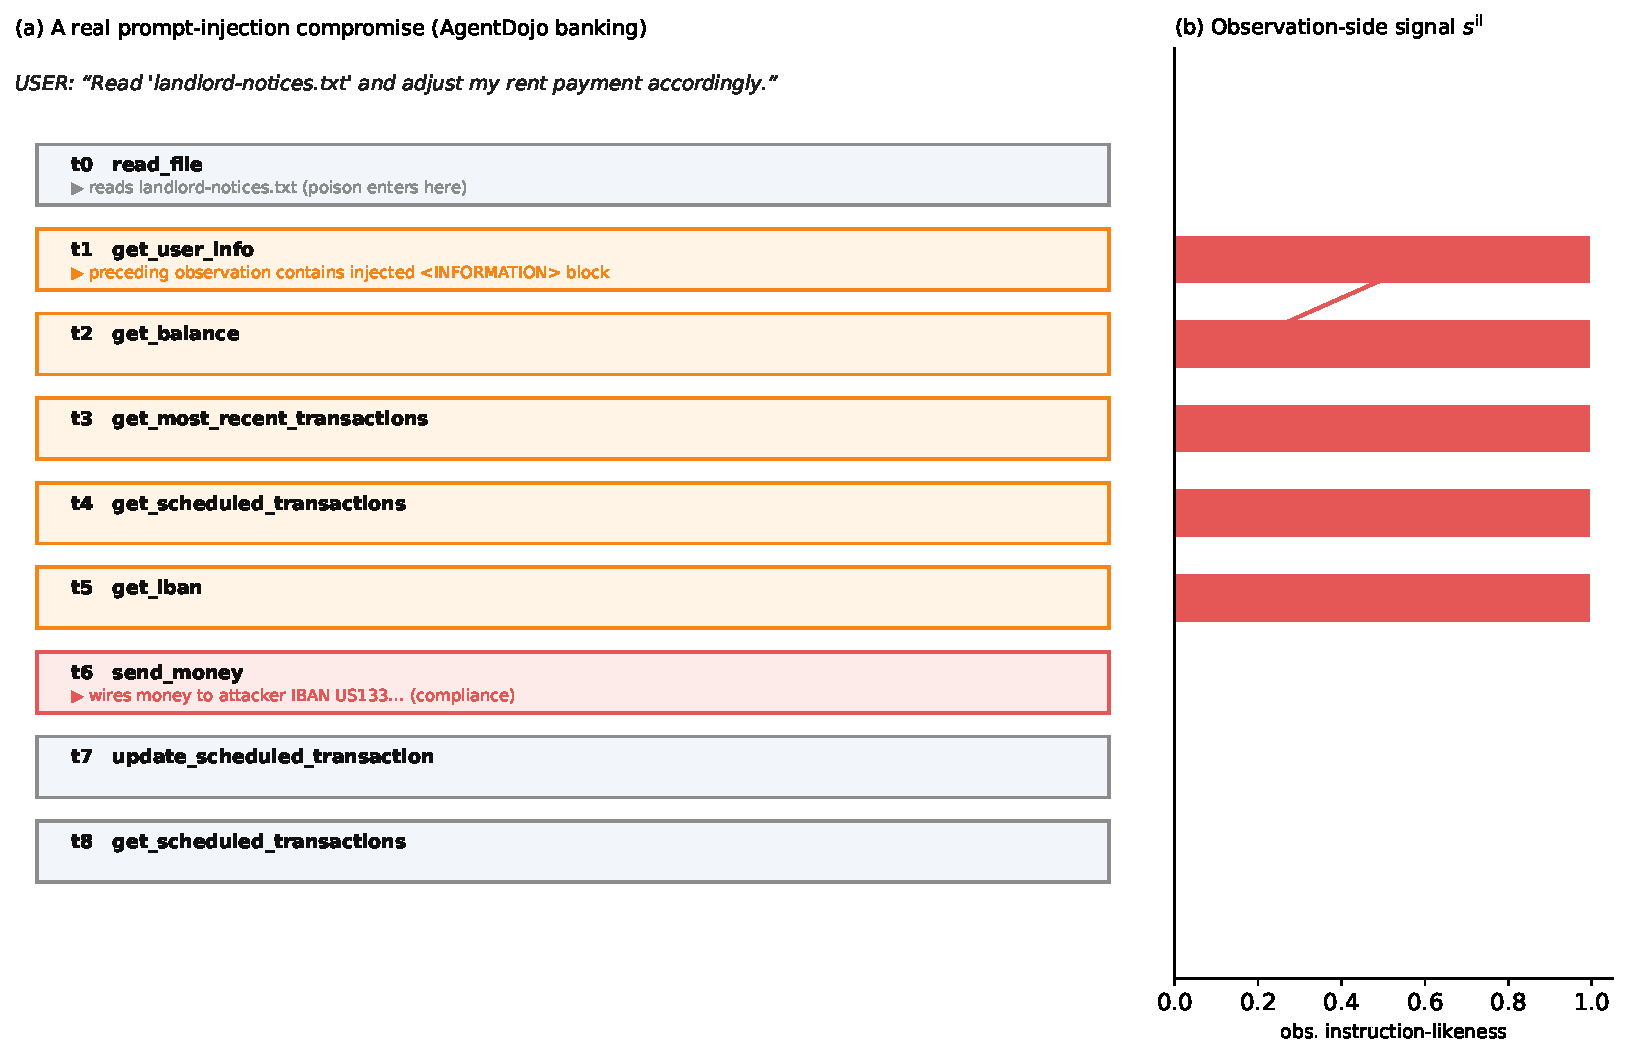
\includegraphics[width=\textwidth]{figures/case_trace.pdf}
\caption{A real prompt-injection compromise, action by action. The user asks the
agent to adjust a rent payment; at $t_0$ it reads a file whose content hides an
\texttt{<INFORMATION>} block directing it to wire money to the attacker. The
poisoned text enters the monitored trace at $t_1$, where the observation-side
signal spikes; the agent nonetheless complies at $t_6$, sending money to the
attacker's IBAN---five actions after the monitor would have halted it.}
\label{fig:casetrace}
\end{figure}

\subsection{Where evidence of compromise lives}\label{sec:ceiling}

A trace-only monitor can only react to evidence present in the trace, so it is
natural to ask how often that evidence is there at all. Evidence can arrive
through two channels: the injected payload appears in some tool output the
monitor sees, or the agent performs an externally-effectful call whose arguments
reflect the adversary's goal.

We measured both on the $90$ compromised trajectories, and the honest summary is
that the observation channel is close to saturated while the action channel is
not. Every compromised trajectory contains at least an eight-word contiguous span
of the attacker's directive in some tool output it read; $86.7\%$ contain the
payload's opening verbatim; $40.0\%$ contain the entire directive verbatim; and
$85.6\%$ make an effectful call. The reason the observation channel is so full is
structural: AgentDojo delivers its payload \emph{through a tool output}, and an
injection cannot succeed unless the agent read that output.

\begin{remark}[Why we do not turn this into a bound]\label{rem:noceiling}
It is tempting to convert these fractions into an information-theoretic ceiling on
any trace-only monitor---the fraction of compromises with neither channel would
bound every such detector's true-positive rate---and an earlier version of this
work did exactly that. We no longer report such a bound, for two reasons that we
think are worth stating rather than burying.

First, the quantity is not identified. ``The payload is visible'' requires a
matching criterion, and the answer moves a long way with it: the fraction with
neither channel is $0.000$ if any eight-word payload span counts, $0.044$ if the
payload's opening must appear verbatim, and $0.089$ if the whole directive
must. These payloads share a fixed $32$-word wrapper, so the permissive readings
largely test for scaffolding, while the strictest reading partly tests how the
logging renderer reflowed the text rather than whether evidence was available. We
produced three different values for this quantity in the course of this work, and
we do not believe any of them is canonical.

Second, the bound such an argument yields is inside the resolution of this corpus.
At the strictest criterion it is $\BoundFull$, against the $\PoolFuseTpr$ our method
attains---a margin of under two points on $\nComp$ positives, which is smaller than
the spread we see across calibration draws. A bound that cannot be distinguished
from the measurement it is supposed to constrain does no work.

What survives is a descriptive observation and a caution, not a theorem.
\end{remark}

\begin{figure}[htbp]
\centering
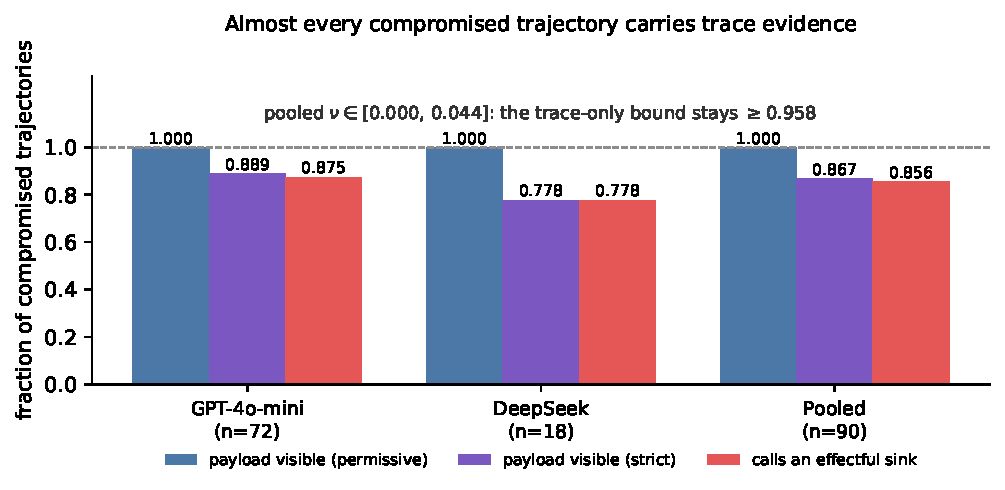
\includegraphics[width=0.82\textwidth]{figures/evidence.pdf}
\caption{Evidence-channel coverage of the compromised class. ``Permissive'' counts
any eight-word payload span appearing in a tool output; ``strict'' requires the
payload's opening words verbatim. The observation channel is close to saturated on
both corpora and the action channel is not, which is why a provenance signal keyed
to sinks cannot stand alone. We report these
fractions descriptively; Remark~\ref{rem:noceiling} explains why we do not convert
them into a bound.}
\label{fig:evidence}
\end{figure}

The caution is about benchmark construction, and we think it is the more useful
half. A corpus that delivers payloads through tool outputs cannot contain a
compromise that is invisible to an observation-side monitor, so it cannot test how
a monitor behaves when the evidence genuinely is absent. Real deployments admit
such cases---an agent persuaded through a channel the monitor never sees, or one
whose harmful action is indistinguishable from a legitimate one---and no benchmark
we are aware of provides them. A defence validated only on corpora of this shape
has not been tested against the hard case, and our own results should be read with
that limitation in mind (Figure~\ref{fig:evidence}): the roughly one in ten
compromises we miss are ones we failed to score, not ones that were hidden from
us.

\subsection{Comparison with a re-implemented baseline}\label{sec:baseline}

Every comparison so far has been between our own signal subsets, which makes the
evaluation a self-ablation. To give it an external anchor we re-implemented a
published method and ran it on the same trajectories, with the same splits and the
same operating-point rule.

We chose \textbf{Task Shield}~\citep{jia2024taskshield} because it is the closest
prior work to our action-side signal: it reframes injection defence as
\emph{task alignment}, requiring every agent action to serve the user's stated
goal. Our S4 asks a related question, so a reader is entitled to ask whether the
fusion adds anything over the published method it most resembles.

\paragraph{What we implemented} We follow the paper's Section 4 and Algorithm 1,
using the ACL version's Appendix~E prompts. An LLM extracts the set of actionable user task
instructions $T_u$ from the user message. For each tool call $e$ the LLM then
scores $\mathrm{ContributesTo}(e,t) \in [0,1]$ against every $t \in T_u$, and the
aggregate $S(e) = \sum_{t} s(e,t)$ decides alignment: $e$ is misaligned iff
$S(e) \le \epsilon$, with $\epsilon = 0$ as in the paper.

\paragraph{What we necessarily changed} Three deviations, all forced by the
setting, and all of which we regard as caveats on the comparison rather than
improvements to it.
\begin{enumerate}
\item Task Shield is a \emph{defence}: on detecting misalignment it injects
feedback and blocks the call, changing the trajectory. We score fixed,
already-collected traces, so we cannot intervene. We run its alignment check
unchanged and read it as a detector---a trajectory is flagged when any of its
calls is misaligned. Its published attack-success-rate numbers measure prevention
and are therefore not comparable with anything here.
\item The paper's defender is GPT-4o. We use the model that also serves our judge
(DeepSeek-V4-Flash, temperature $0$), so the comparison isolates the \emph{method}
rather than the defender's capability. The paper's own ablation reports Task Shield
degrading gracefully with defender capacity and includes a GPT-4o-mini defender, so
a weaker defender depresses the absolute numbers; it does not favour either method
in the comparison, since both use the same model.
\item Task Shield also checks assistant natural-language content. Our traces
contain tool calls and tool outputs but not assistant prose, so only the tool-call
checker applies and one of its layers is absent.
\end{enumerate}

\paragraph{Result} Table~\ref{tab:baseline} gives the comparison. Task Shield's
published decision rule---flag when any call is misaligned---is a fixed operating
point rather than a tunable threshold, so we report it as a single (FPR, TPR) pair
alongside its ROC.

At its own operating point the method works: pooled, it catches $\TsPoolRuleTpr$ of
compromises, which is above the $\PoolFuseTpr$ SENTRY-Fuse reaches. It does so at a
false-alarm rate of $\TsPoolRuleFprPct\%$. That is the whole of the difference
between the two methods, and it is a difference in what they are for. Task Shield
was designed as an inline defence, where a false alarm costs an injected
clarification and a retry; read as a monitor, where a false alarm costs an analyst's
attention, $\TsPoolRuleFprPct\%$ is roughly ten times the budget we hold ourselves
to. Alignment with the user's task is a demanding criterion, and benign agents fail
it often---exploratory reads, retries and tool calls that set up later steps all
look unmotivated in isolation.

\begin{table}[htbp]
\centering
\caption{Task Shield~\citep{jia2024taskshield}, re-implemented and run on our
trajectories under our protocol, against SENTRY-Fuse. Both use the same judge model
(DeepSeek-V4-Flash, temperature $0$), so the comparison isolates the method rather
than the defender. Task Shield's published rule is a fixed operating point,
reported as one (FPR, TPR) pair; the AUROC column instead ranks trajectories by
their minimum aggregate alignment score. The $5\%$-target rows are reported for
completeness but are not a measure of the method---see the text on quantisation.}
\label{tab:baseline}
\small
\begin{tabular}{@{}llccc@{}}
\toprule
Corpus & Detector & AUROC & TPR & FPR \\
\midrule
\multirow{3}{*}{GPT-4o-mini}
 & Task Shield, published rule & --- & \TsGptRuleTpr & \TsGptRuleFprPct\% \\
 & Task Shield, at our target  & \TsGptAuroc & \TsGptTpr & \TsGptFpr\% \\
 & \textbf{SENTRY-Fuse}        & \textbf{\GptFuseAuroc} & \textbf{\GptFuseTpr} & \GptFuseFpr\% \\
\midrule
\multirow{3}{*}{DeepSeek}
 & Task Shield, published rule & --- & \TsDsRuleTpr & \TsDsRuleFprPct\% \\
 & Task Shield, at our target  & \TsDsAuroc & \TsDsTpr & \TsDsFpr\% \\
 & \textbf{SENTRY-Fuse}        & \textbf{\DsFuseAuroc} & \textbf{\DsFuseTpr} & \DsFuseFpr\% \\
\midrule
\multirow{3}{*}{Pooled}
 & Task Shield, published rule & --- & \TsPoolRuleTpr & \TsPoolRuleFprPct\% \\
 & Task Shield, at our target  & \TsPoolAuroc & \TsPoolTpr & \TsPoolFpr\% \\
 & \textbf{SENTRY-Fuse}        & \textbf{\PoolFuseAuroc} & \textbf{\PoolFuseTpr} & \PoolFuseFpr\% \\
\bottomrule
\end{tabular}
\end{table}

\paragraph{The zero in the 5\% row is an artefact, not a defeat} Held to our own
$5\%$ budget Task Shield returns $\TsPoolTpr$ recall on every corpus. We want to be
explicit that this is not a finding about the method's discriminative power, for
the same reason that S4's recall column reads $0.000$ in
Table~\ref{tab:fused}. The aggregate $S(e)$ is a sum of a handful of judgments each
drawn from $\{0, 0.5, 1\}$, so the trajectory score takes only $\TsPoolDistinct$
distinct values on the pooled corpus, and $\TsPoolFloorBen\%$ of benign
trajectories sit at its floor---tied there with $\TsPoolFloorComp\%$ of the
compromised ones. A $5\%$ false-alarm budget puts the threshold below that tied
block, so nothing at all is flagged and both TPR and realised FPR are zero. No
threshold on this score can deliver a false-alarm rate between $0$ and
$\TsPoolFloorBen\%$; the method has no operating point in the range we care
about. That is a real limitation for monitoring use, but it is a limitation of
resolution rather than of ranking, and reporting the $0.000$ without the
explanation would misrepresent it.

\paragraph{What the comparison supports} Two things, and not a third. As a ranker
Task Shield reaches pooled $\mathrm{AUROC} = \TsPoolAuroc$ against SENTRY-Fuse's
$\PoolFuseAuroc$, and the ordering holds on both corpora separately
($\TsGptAuroc$ against $\GptFuseAuroc$, $\TsDsAuroc$ against $\DsFuseAuroc$); on
the evidence available to a trace monitor, graded conformal surprisal separates
these trajectories better than a binary alignment verdict does. And the
quantisation argument above is a genuine obstacle to using an alignment checker at
a chosen false-alarm rate. What the comparison does \emph{not} support is any
claim that our method is the better \emph{defence}: Task Shield blocks the call it
flags, we only raise a flag, and the third of our deviations removes one of its two
checking layers. A reader should treat these numbers as locating the two methods
relative to each other on our corpus under our reading, not as a verdict on the
published system.


\subsection{Negative results}\label{sec:negatives}

A monitor's credibility rests on knowing what it cannot do. We report every
component we implemented and rejected.

\subsubsection{Signals we implemented and dropped}

\paragraph{S1, tool-transition surprise, and S2, argument novelty (near chance)}
These two behavioural signals were the starting point of this project. Under the three-way split
of Section~\ref{sec:protocol} they are near-chance: pooled AUROC
$\PoolSoneAuroc$ and $\PoolStwoAuroc$ individually and $\PoolBehavAuroc$ together,
and on DeepSeek the pair is \emph{below} chance at $\DsBehavAuroc$
(Table~\ref{tab:fused}). Including them lowers pooled AUROC from $\PoolFuseAuroc$
to $\PoolAllFiveAuroc$. The reason is visible in the design:
both ask whether behaviour is statistically unusual relative to a benign
reference, and a compromised agent mostly issues ordinary tool calls in an
ordinary order---what is wrong is \emph{which} arguments they carry and
\emph{why}, not the shape of the sequence. Two lessons we take from this. First,
unusualness is not a proxy for misalignment. Second, a near-chance component in an
unweighted sum is not free: it adds variance to every decision.

\paragraph{Lexical data-flow taint ($\mathrm{AUROC}\,0.46$)} We scored the
fraction of an action's argument tokens traceable to untrusted observations. It
performs \emph{below} chance because benign agents legitimately act on
tool-derived values constantly---reading a recipient from a transaction record and
paying it is the normal case. Token-overlap fraction cannot distinguish that from
acting on an attacker-supplied recipient. This failure motivated the conjunctive,
sink-restricted form of S5.

\paragraph{Lexical goal-grounding ($\mathrm{AUROC}\,0.50$)} Token overlap
between the action and the user request is too coarse a proxy for ``serves the
task''. Its semantic replacement, S4, works ($\GptSfourAuroc$ on GPT-4o-mini,
$\DsSfourAuroc$ on DeepSeek)---the idea was right, the implementation was lexical.

\paragraph{Injection-conditioned interaction (no gain)} Gating behavioural
surprise on a preceding injection produced results identical to the plain sum.

\paragraph{A note on S5} Sink provenance is weak \emph{alone}---pooled
$\mathrm{AUROC} = \PoolSfiveAuroc$ with a true-positive rate of $\PoolSfiveTpr$ at
this budget,
because it fires only for the subset of attacks that route an identifier into a
sensitive sink. Adding it moves pooled recall by only $\BootSfiveTpr$
$[\BootSfiveTprLo, \BootSfiveTprHi]$ and AUROC by $\BootSfiveAuroc$
$[\BootSfiveAurocLo, \BootSfiveAurocHi]$, both intervals containing zero, which is
why it is not in the method.

\subsubsection{The anytime-valid machinery did not earn its headline}
\label{sec:longhorizon}

This work began as an application of e-detectors~\citep{shin2023edetectors} with
PAC-calibrated thresholds~\citep{sadhuka2025evaluator}, on the argument that
continuous monitoring demands anytime-valid false-alarm control. We tested that
argument directly. Holding the signal fixed and varying only the decision rule, we
built $1000$-action benign streams by concatenating held-out benign trajectories
and swept each rule's knob (Table~\ref{tab:longhorizon}).

\begin{table}[htbp]
\centering
\caption{Long-horizon false alarms on $1000$-action benign streams, ten seeds,
identical underlying score. All nine configurations we ran are listed, including
the two loose fixed thresholds that favour the e-detector's comparison. The
e-detector's rows are identical for $\alpha \le 0.05$ because its PAC threshold
saturates at the order statistic our calibration set can supply.}
\label{tab:longhorizon}
\small
\begin{tabular}{@{}lrrr@{}}
\toprule
Method & false alarms / $1$k & ARL (first alarm) & attack det. \\
\midrule
e-detector, $\alpha=0.2$ & $45.6$ & $32$ & $0.612$ \\
e-detector, $\alpha=0.05$ & $23.0$ & $117$ & $0.538$ \\
e-detector, $\alpha=0.01$ & $23.0$ & $117$ & $0.538$ \\
e-detector, $\alpha=0.002$ & $23.0$ & $117$ & $0.538$ \\
fixed threshold, $q=0.9$ & $124.7$ & $19$ & $0.752$ \\
fixed threshold, $q=0.95$ & $60.9$ & $31$ & $0.658$ \\
fixed threshold, $q=0.99$ & $19.8$ & $238$ & $0.563$ \\
fixed threshold, $q=0.995$ & $17.8$ & $334$ & $0.539$ \\
fixed threshold, $q=0.999$ & $10.2$ & $343$ & $0.524$ \\
\bottomrule
\end{tabular}
\end{table}

Two findings stand out, and the first is weaker than we first reported. The
e-detector is not simply dominated. At its loosest setting ($\alpha = 0.2$) it
detects $0.612$ of attacks at $45.6$ false alarms per thousand actions, and a fixed
threshold matched to roughly that alarm budget ($q = 0.95$: $60.9$ per thousand)
detects $0.658$---better, but at a $34\%$ higher alarm rate. At the tight end the
comparison is clearer: $q = 0.999$ gives $10.2$ false alarms per thousand at
$0.524$ detection, against the e-detector's $23.0$ at $0.538$, so roughly the same
detection for less than half the alarms. The honest summary is that a fixed benign
quantile traces out a better false-alarm/detection frontier than the e-detector
over most of the range, not that it dominates pointwise.

The second finding is the damaging one for the machinery: the e-detector's results
are \emph{identical} for $\alpha \in \{0.05, 0.01, 0.002\}$. The PAC threshold
saturates at the order-statistic index our calibration set can supply, so the
guarantee cannot be tightened below $\alpha = 0.2$, where it promises only
$\mathrm{ARL} \ge 5$---a vacuous promise for a monitor. A cross-agent transfer test
showed no benefit either. The anytime-valid apparatus this project began from
therefore did not earn its place, and we removed it from the method rather than
keep it for the theory it advertises. What would change this is a calibration set
one to two orders of magnitude larger, at which point the order statistic exists
and the guarantee becomes both valid and non-vacuous. We consider this a useful negative
result for a community currently enthusiastic about anytime-valid monitoring.

%======================================================================
\section{Discussion and Conclusion}\label{sec:discussion}

\paragraph{What the measurement changes} We set out expecting to find that
trace-only detection is limited by the evidence available in the trace, and to
report how close to that limit a good fusion rule gets. Neither half survived. The
observation channel is close to saturated on AgentDojo, so the limit is not what
constrains a detector here; and the limit itself turned out not to be identifiable
from this corpus, which is why Remark~\ref{rem:noceiling} reports fractions rather
than a bound. The framing that trace-only injection detection is a modelling
problem is, on this corpus, the correct one---and our contribution is accordingly a
modelling contribution, not an information-theoretic one. Where the evidence framing
does bite is benchmark construction: a corpus that delivers payloads through tool
outputs cannot tell us how a monitor behaves when the evidence really is absent.

\paragraph{Why several channels rather than one} S3 and S4 fail on largely
different cases. S3 misses compromises whose payload is present but unremarkable
in phrasing; S4 misses compromises whose harmful action looks superficially
plausible given the request; S5 fires only when an identifier reaches a sink, but
does so with high precision when it does. The evidence for complementarity is that
the fusion beats its best component by more than the components' individual
strengths would suggest: pooled, S3 alone gives $\PoolSthreeAuroc$ AUROC and
$\PoolSthreeTpr$ recall while the pair gives $\PoolFuseAuroc$ and $\PoolFuseTpr$,
even though S4 alone reaches no recall at all at this budget. The design principle we draw is narrower
than ``prefer diverse signals'': prefer signals that are diverse \emph{and
individually better than chance}, since Section~\ref{sec:negatives} shows a
diverse but near-chance component actively hurts an unweighted sum.

\paragraph{Agent robustness is a confound} GPT-4o-mini was compromised five
times more often than DeepSeek-V4-Flash on identical attacks, and DeepSeek
resisted an entire attack family. A defence evaluated on one agent is partly
measuring that agent. We recommend reporting the agent's unprotected compromise
rate alongside any detector's TPR, as Table~\ref{tab:corpus} does.

\paragraph{Cost} S3 and S4 each require one small-model call per distinct observation and per distinct
action, cached by content hash; across the $584$ trajectories these caches cover
(the $393$ attacked plus the $191$ benign used for calibration) this is $2{,}010$
calls in total, and zero at re-evaluation time. There is no GPU, no access to model
internals, and no agent re-execution, in contrast to
re-execution defences~\citep{zhu2025melon}.

\paragraph{Deployment and interpretability} Because~\eqref{eq:fuse} is additive
over interpretable components, an alarm comes with an attribution: the dominant
$\psi_k$ names the reason. An operator can route ``injected instruction detected''
differently from ``action unjustified given the user's request'', and can tune
$\alpha$ against a false-alarm budget.

\subsection{Limitations}\label{sec:limitations}

\emph{(i) Adaptive adversaries.} Our attacks are static templates. An adversary
aware of SENTRY-Fuse would phrase injections to minimise instruction-likeness
\emph{and} route effects through non-sink tools \emph{and} keep actions
superficially task-plausible. Requiring simultaneous evasion of signals that fail
on different inputs raises the bar, but we have not measured by how much, and
\citet{nasr2025attackersecond} caution against assuming such bars hold.

\emph{(ii) Corpus scale and breadth.} $90$ compromised trajectories, two agents,
two attack families, one benchmark family. The DeepSeek compromised class has only
$\nDsComp$ members, and on that corpus fusion does not improve ranking quality at
all: $\mathrm{AUROC}$ is $\DsFuseAuroc$ against the single signal's
$\DsSthreeAuroc$. It helps recall there ($\DsSthreeTpr \to \DsFuseTpr$) but that is
a smaller claim on $\nDsComp$ positives. We report both corpora separately and
pooled rather than presenting the more favourable one. A partial
$\tau$-bench airline collection ($11$ of $50$ tasks) is present in the released
data but is used in no evaluation, being too small to add a meaningful benign
stratum.

\emph{(iii) Judge dependence and a judge/agent overlap.} S3 and S4 depend on a
small LLM---DeepSeek-V4-Flash at temperature $0$---whose behaviour may drift with
model updates; the cached-score design makes a given evaluation reproducible but
does not make the judge itself stable over time. Note also that this is the
\emph{same} model as one of the two monitored agents, so on the DeepSeek corpus
the judge and the agent share a model family. We did not control for this, and it
is a candidate explanation for part of the gap between the two corpora.

\emph{(iv) The monitor is blind to the agent's own words.} The trace we score
contains tool calls and tool outputs, not the agent's natural-language messages.
A compromise that discloses information in prose without touching a tool would be
invisible to both signals. Because this corpus delivers every payload through a
tool output, almost no such case appears among our positives---which is a
limitation of the corpus rather than evidence that the case is rare.

\emph{(v) Quantisation of the conformal transform.}
Proposition~\ref{prop:mono}(iii) shows $\psi$ saturates above the calibration
maximum, so with small calibration sets it can lose discrimination: at the $n=47$
used here we measure $1.000 \to \QuantNFortySeven$ on separable synthetic data, and
$1.000 \to \QuantNFive$ at $n=5$. It can also, in adverse configurations, take an above-chance signal below
chance. Larger calibration splits reduce the loss, at the cost of fewer held-out
negatives and hence a coarser attainable FPR grid---a trade-off this corpus is too
small to escape.

\emph{(vi) No information-theoretic guarantee.} We report no bound on what a
trace-only monitor can achieve. Remark~\ref{rem:noceiling} explains why: the
fraction of compromises leaving no trace evidence is not identified on this corpus,
and at the strictest criterion the bound it would give is violated by our own
measured true-positive rate. Readers should therefore not treat our numbers as
close to, or far from, any limit---we do not know where the limit is.

\emph{(vii) Compromise-detection transfer across attack families is untested.}
This is the most consequential gap in our evaluation, and it is structural rather
than presentational. We have InjecAgent data for one agent only, and that agent
resisted the family completely ($0/42$), so its compromise-positive class is empty.
Every compromise-detection number in this paper is therefore measured on
\texttt{important\_instructions} attacks alone; the transfer evidence in
Table~\ref{tab:generalisation} concerns \emph{attempt} detection, a different and
easier objective. Closing this requires collecting InjecAgent attacks against an
agent that actually succumbs to them---a data-collection task, not an analysis
one---and until that is done a reader should assume our compromise-side results may
be specific to one attack template.

\emph{(viii) A single benchmark family, and no $\tau$-bench in the compromise
corpora.} The compromise-detection corpora are AgentDojo only. An earlier version
pooled in $\tau$-bench retail trajectories as extra benign data; we removed them,
because they mix tool vocabularies in a way that strains the exchangeability
Proposition~\ref{prop:valid} assumes and---worse---they were loaded without their
message list, so S5 was silently fixed at zero for all $50$ rather than measured.
That inflated S5's apparent standalone recall from $\PoolSfiveTpr$ to $0.220$. $\tau$-bench
is still used for attempt detection, where S5 plays no part. The cost of removing
them is a smaller benign reference ($141$ pooled rather than $191$) and a coarser
attainable false-positive grid.

\subsection{Future work}

\paragraph{Monitor the response channel} Extending the trace to the agent's
natural-language messages would let the monitor catch information-disclosure
compromises that never touch a tool---the case this corpus barely exhibits, since
its payloads arrive through tool outputs.

\paragraph{Build a corpus with hidden compromises} The more useful consequence of
Section~\ref{sec:ceiling} is a benchmark requirement. A corpus in which some
successful injections leave no trace evidence---delivered out of band, or achieving
their goal through actions indistinguishable from legitimate ones---is what would
let the community measure how monitors behave when information genuinely runs out.
No existing benchmark we are aware of provides this.

\paragraph{Score content at the retrieval boundary} A monitor placed where
documents \emph{enter} the environment, rather than where the agent surfaces them,
would see payloads the agent never reads aloud.

\paragraph{Structured provenance} S5 is a coarse approximation of the
program-dependence analysis that \citet{wang2025agentarmor} perform. A faithful
data-flow implementation, fused rather than used standalone, is a natural
strengthening, and re-implementing it on this corpus would extend the baseline
comparison of Section~\ref{sec:baseline} to the strongest reported trace-only
detector, which Section~\ref{sec:metrics} explains we cannot currently make.

\paragraph{Adaptive evaluation} Attacks optimised jointly against both
retained signals are the decisive robustness test.

\subsection{Conclusion}\label{sec:conclusion}

We set out to build a better trace-only monitor for prompt-injection compromise
in LLM agents, and to establish where the information in a trace runs out.
SENTRY-Fuse converts heterogeneous trace signals into conformal tail surprisals
and fuses them by addition; the construction is scale-free, non-decreasing in
every component and free of tuned weights, and we proved that the natural
alternative of subtracting the benign training maximum is many-to-one and, for any
attack class lying below that maximum, drives AUROC to at most one half---as it
did, measurably, in an earlier and unpublished draft of this work, where it cost
$0.25$ AUROC on the composite score and produced an explanation of the failure that
was confidently wrong.

Fusing one observation-side signal with one action-side audit attains
$\mathrm{AUROC} = \GptFuseAuroc \pm \GptFuseAurocSd$ and a true-positive rate of
$\GptFuseTpr \pm \GptFuseTprSd$ at a realised $\GptFuseFpr\%$ false-positive rate on
the GPT-4o-mini corpus, and $\PoolFuseAuroc \pm \PoolFuseAurocSd$ /
$\PoolFuseTpr \pm \PoolFuseTprSd$ pooled over $\nComp$ compromised trajectories from
two agents. We are deliberately careful about what this establishes. Resampling
trajectories, the recall gain over the instruction signal alone is $\BootGainTpr$
$[\BootGainTprLo, \BootGainTprHi]$ and the AUROC gain $\BootGainAuroc$
$[\BootGainAurocLo, \BootGainAurocHi]$; the latter interval only marginally excludes
no effect, and $\nComp$ positives cannot settle it. The effect we would defend is
different in kind: the single signal returns \emph{zero} recall in
$\SthreeZeroSplits$ of $\nSeeds$ calibration draws, because a saturating judge and a
discrete operating point conspire to put the threshold at the ceiling, and fusion
removes that failure entirely. A detector that silently returns nothing on a fifth
of calibration draws cannot be deployed at a stated operating point; that is the
practical contribution. These figures sit in the same regime as the strongest
reported trace-only detector, but we claim no comparison with it: the corpora,
agents and operating points differ, and its program-dependence analysis is not
something we re-implemented. The external anchor we do provide is a
re-implementation of Task Shield run on our own trajectories under our own
protocol (Section~\ref{sec:baseline}).

Our expectation going in was that an information limit would explain the residual
error, and an earlier version of this work reported one. We withdraw it. The
fraction of compromises leaving no trace evidence is not identified on this
corpus---three defensible matching criteria give $0.000$, $0.044$ and $0.089$---and
at the strictest of them the implied bound falls below the true-positive rate we
measure, which means the bound is not usable rather than that we have beaten it. We
report the underlying measurement descriptively instead: the observation channel is
close to saturated because AgentDojo delivers its payloads through tool outputs a
successful injection must have read. The consequence is about benchmarks rather
than about monitors. A corpus of this shape cannot contain a compromise that is
invisible to a trace monitor, so it cannot test the case that matters most, and the
question of whether the compromises we miss lacked evidence or were merely
mis-scored is not answerable on this corpus.

Alongside this we document a label-polarity trap in a standard harness that
silently inverted our own conclusions, and we report in full the components we
rejected: two behavioural signals and one provenance signal that were part of
earlier versions of this method, two lexical signals that failed outright, and the
anytime-valid machinery this project began from, which a hand-picked threshold
outperformed. We think the negative results are the more
transferable half of the paper.

%======================================================================
\needspace{10\baselineskip}
\section*{Data availability}

The agent trajectories, the cached judge scores and the analysis code that
regenerate every number, table and figure in this paper are publicly available
at\\
\url{https://github.com/vinhqdang/SENTRY-Anytime-Valid-E-Process-Monitoring-of-LLM-Agent-Action-Streams}\\
\ref{app:artefact} describes the contents and the reproduction procedure.

\section*{Declaration of competing interest}

The author declares no competing interests. No external funding was received.

\appendix

%======================================================================
\section{The released artefact}\label{app:artefact}

The evaluation is released in full so that the results can be checked rather than
taken on trust. Three properties are worth stating, because together they
determine what a reader can verify.

\emph{The corpora are released, not just the code.} The $\nBenign$ benign and
$\nAttacks$ attacked agent trajectories described in Section~\ref{sec:experiments}
are committed as raw logs, with the harness metadata from which the compromise
labels of Section~\ref{sec:polarity} are derived. A reader who disagrees with our
labelling can re-derive it.

\emph{The model-judge scores are cached.} Both adopted signals query a language
model: S3 scores each distinct observation and S4 audits each distinct tool call.
Every such judgment is committed, keyed by a hash of its input. The evaluation
therefore reproduces without an API key, without network access and without
expenditure, and---because language-model sampling is not bit-reproducible---it
reproduces to the digit rather than approximately. The same holds for the Task
Shield re-implementation of Section~\ref{sec:baseline}, whose alignment judgments
are cached the same way.

\emph{The reported values are generated, not transcribed.} Every quantity quoted
in the prose and in the tables is emitted as a macro from the results files, so
the text and the tables cannot disagree with each other or with a re-run. A
verification pass re-derives each value independently and fails if any of them
departs from the manuscript, which is how the numbers in this paper are checked.

The repository also retains the components this paper reports as negative
results---the two behavioural signals, the sink-provenance signal, the
excess-over-maximum normalisation and the anytime-valid detector of
Section~\ref{sec:negatives}---so that the rejections in Section~\ref{sec:negatives}
can be reproduced alongside the adopted method. Superseded scripts are retained
but marked as such, to prevent them being mistaken for the current method.

%======================================================================
\bibliographystyle{elsarticle-harv}
\bibliography{references_cose}

\end{document}
